\documentclass[a4paper]{article}

%% Language and font encodings
\usepackage[english]{babel}
\usepackage[utf8]{inputenc}
\usepackage[T1]{fontenc}
\usepackage[section]{placeins}
\usepackage{graphicx}
\usepackage{caption}
\usepackage{subcaption}
\usepackage{float}
\usepackage{verbatim}
\usepackage{color,soul}
\usepackage[backend=biber,style=ieee]{biblatex}
\addbibresource{main.bib}


%% Sets page size and margins
\usepackage[a4paper,top=3cm,bottom=2cm,left=3cm,right=3cm,marginparwidth=1.75cm]{geometry}

%% Useful packages
\usepackage{amsmath}
\usepackage{graphicx}
\usepackage[colorinlistoftodos]{todonotes}
\usepackage[colorlinks=true, allcolors=blue]{hyperref}
\usepackage{listings}
\usepackage{color} %red, green, blue, yellow, cyan, magenta, black, white
\definecolor{mygreen}{RGB}{28,172,0} % color values Red, Green, Blue
\definecolor{mylilas}{RGB}{170,55,241}

\makeatletter
\newcommand{\filecaption}[1]{\filename@parse{#1}\filename@base.\filename@ext}
\makeatother

\newcommand{\filelisting}[2][]{%
	\lstinputlisting[caption={\texttt{\protect\filecaption{\detokenize{#2}}}},#1]{#2}%
}

\newcommand{\code}[1]{\texttt{\detokenize{#1}}}

\title{ECE 271 Design Project, Group 3}
\author{Casey Huggins, Raymond Jung, Matthew Macovsky, Patrick McGrath}
\date{June 6th, 2019}

\begin{document}

\lstset{language=Verilog,%
    basicstyle=\tiny \color{red},
    breaklines=true,%
    keywordstyle=\color{blue},%
    morekeywords=[2]{1}, keywordstyle=[2]{\color{black}},
    identifierstyle=\color{black},%
    stringstyle=\color{mylilas},
    commentstyle=\color{mygreen},%
    showstringspaces=false,%without this there will be a symbol in the places where there is a space
    numbers=left,%
    numberstyle={\tiny \color{black}},% size of the numbers
    numbersep=9pt, % this defines how far the numbers are from the text
    emph=[1]{for,end,break},emphstyle=[1]\color{red}, %some words to emphasise
    %title=\lstname
}

\maketitle
\tableofcontents
\newpage
\section{Introduction}

\paragraph{The purpose of this project is to design and implement decoders which interpret the inputs of different devices, each device using different clock speeds, timings, and protocols for representing their data. The three device protocols supported in this project were: the PS/2 protocol, which may be used by a keyboard, the IR communication protocol, more specifically the data for an infrared remote control, and lastly, the famous NES controller and its communication protocol. In order to improve the functionality of this project, all three of these controllers will be supported and their respective decoders will be connected to the output by way of a multiplexer. It will then be left up to the interpretation of the receiver for how to handle and interpret the outputs of these circuits.}

\subsection{Project deliverables}
\begin{itemize}
\item Decodes controller inputs from IR VCR remote, NES controller, and PS2 keyboard protocols.
\item (Extra feature) Allows user to select which controller they wish to have interpreted by the circuit.
\end{itemize}

\newpage
\section{High Level Description}

The project consists of three decoders, one each for NES, IR, and PS2 controllers, which all forward their outputs to a multiplexer. The multiplexer has a 2-bit input which allows for it to select between the three different controllers' inputs. The 8-bit output of the multiplexer is then wired to the output of the circuit. 

\begin{figure}[ht]
  \centering
    
\includegraphics[width=.5\textwidth]{images/block_diagrams/top_level.png}
	\caption{The top level design for this project.}
    \label{fig:top_level}
\end{figure}

\subsection{Devices Mux}

\textbf{Input:} This module reads values from each of the three device blocks (\code{i_nes}, \code{i_ps2}, \code{i_vcr}) as well as a default value (\code{i_default}).  It also reads a select input (\code{i_sel}).
\\ \\
\textbf{Output:} \code{o_selection} is one of the input values, selected depending on \code{i_sel}.
\\ \\
The code for this block is given in \autoref{lst:sv_devices_mux}.

\begin{figure}[H]
	\centering
	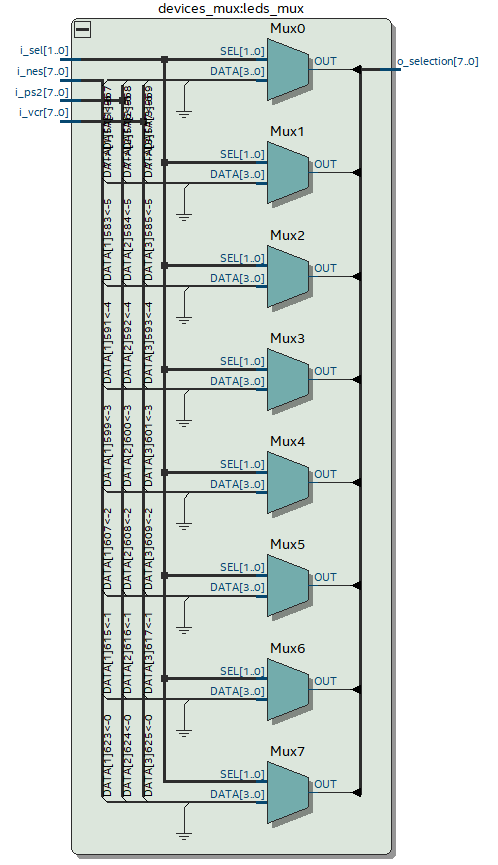
\includegraphics[width=.85\textwidth]{images/block_diagrams/devices_mux.png}
	\caption{An expanded view of the \code{devices_mux} block \code{leds_mux} in \autoref{fig:top_level}.  This module uses muxes to select which device to send to the FPGA outputs based on \code{i_sel}.  In this particular instance, \code{i_default} was connected to 0, so it was simplified from being a separate input to being connections within the module to GND.  The \code{i_sel} value \code{00} connects \code{o_selection} to \code{i_default}; \code{01} connects it to \code{i_nes}; \code{10} connects it to \code{i_ps2}; and \code{11} connects it to \code{i_vcr}.}
	\label{fig:block_vcr_devices_mux}
\end{figure}

\begin{figure}[H]
	\centering
	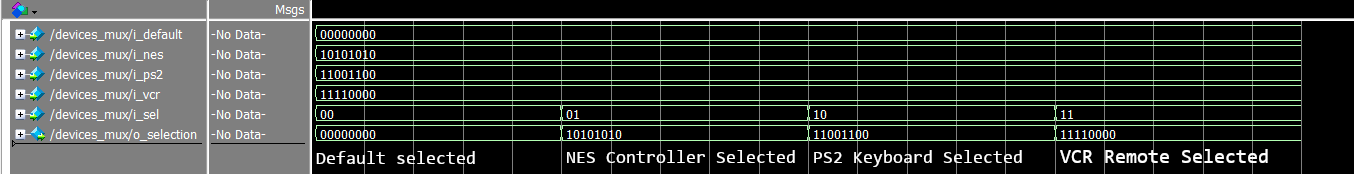
\includegraphics[width=.95\textwidth]{images/sim/devices_mux.png}
	\caption{Simulation results for the \code{devices_mux} module (see \autoref{lst:sim_devices_mux} for simulation code).}
\end{figure}

\subsection{NES Controller Reader}

\begin{figure}[H]
  \centering
    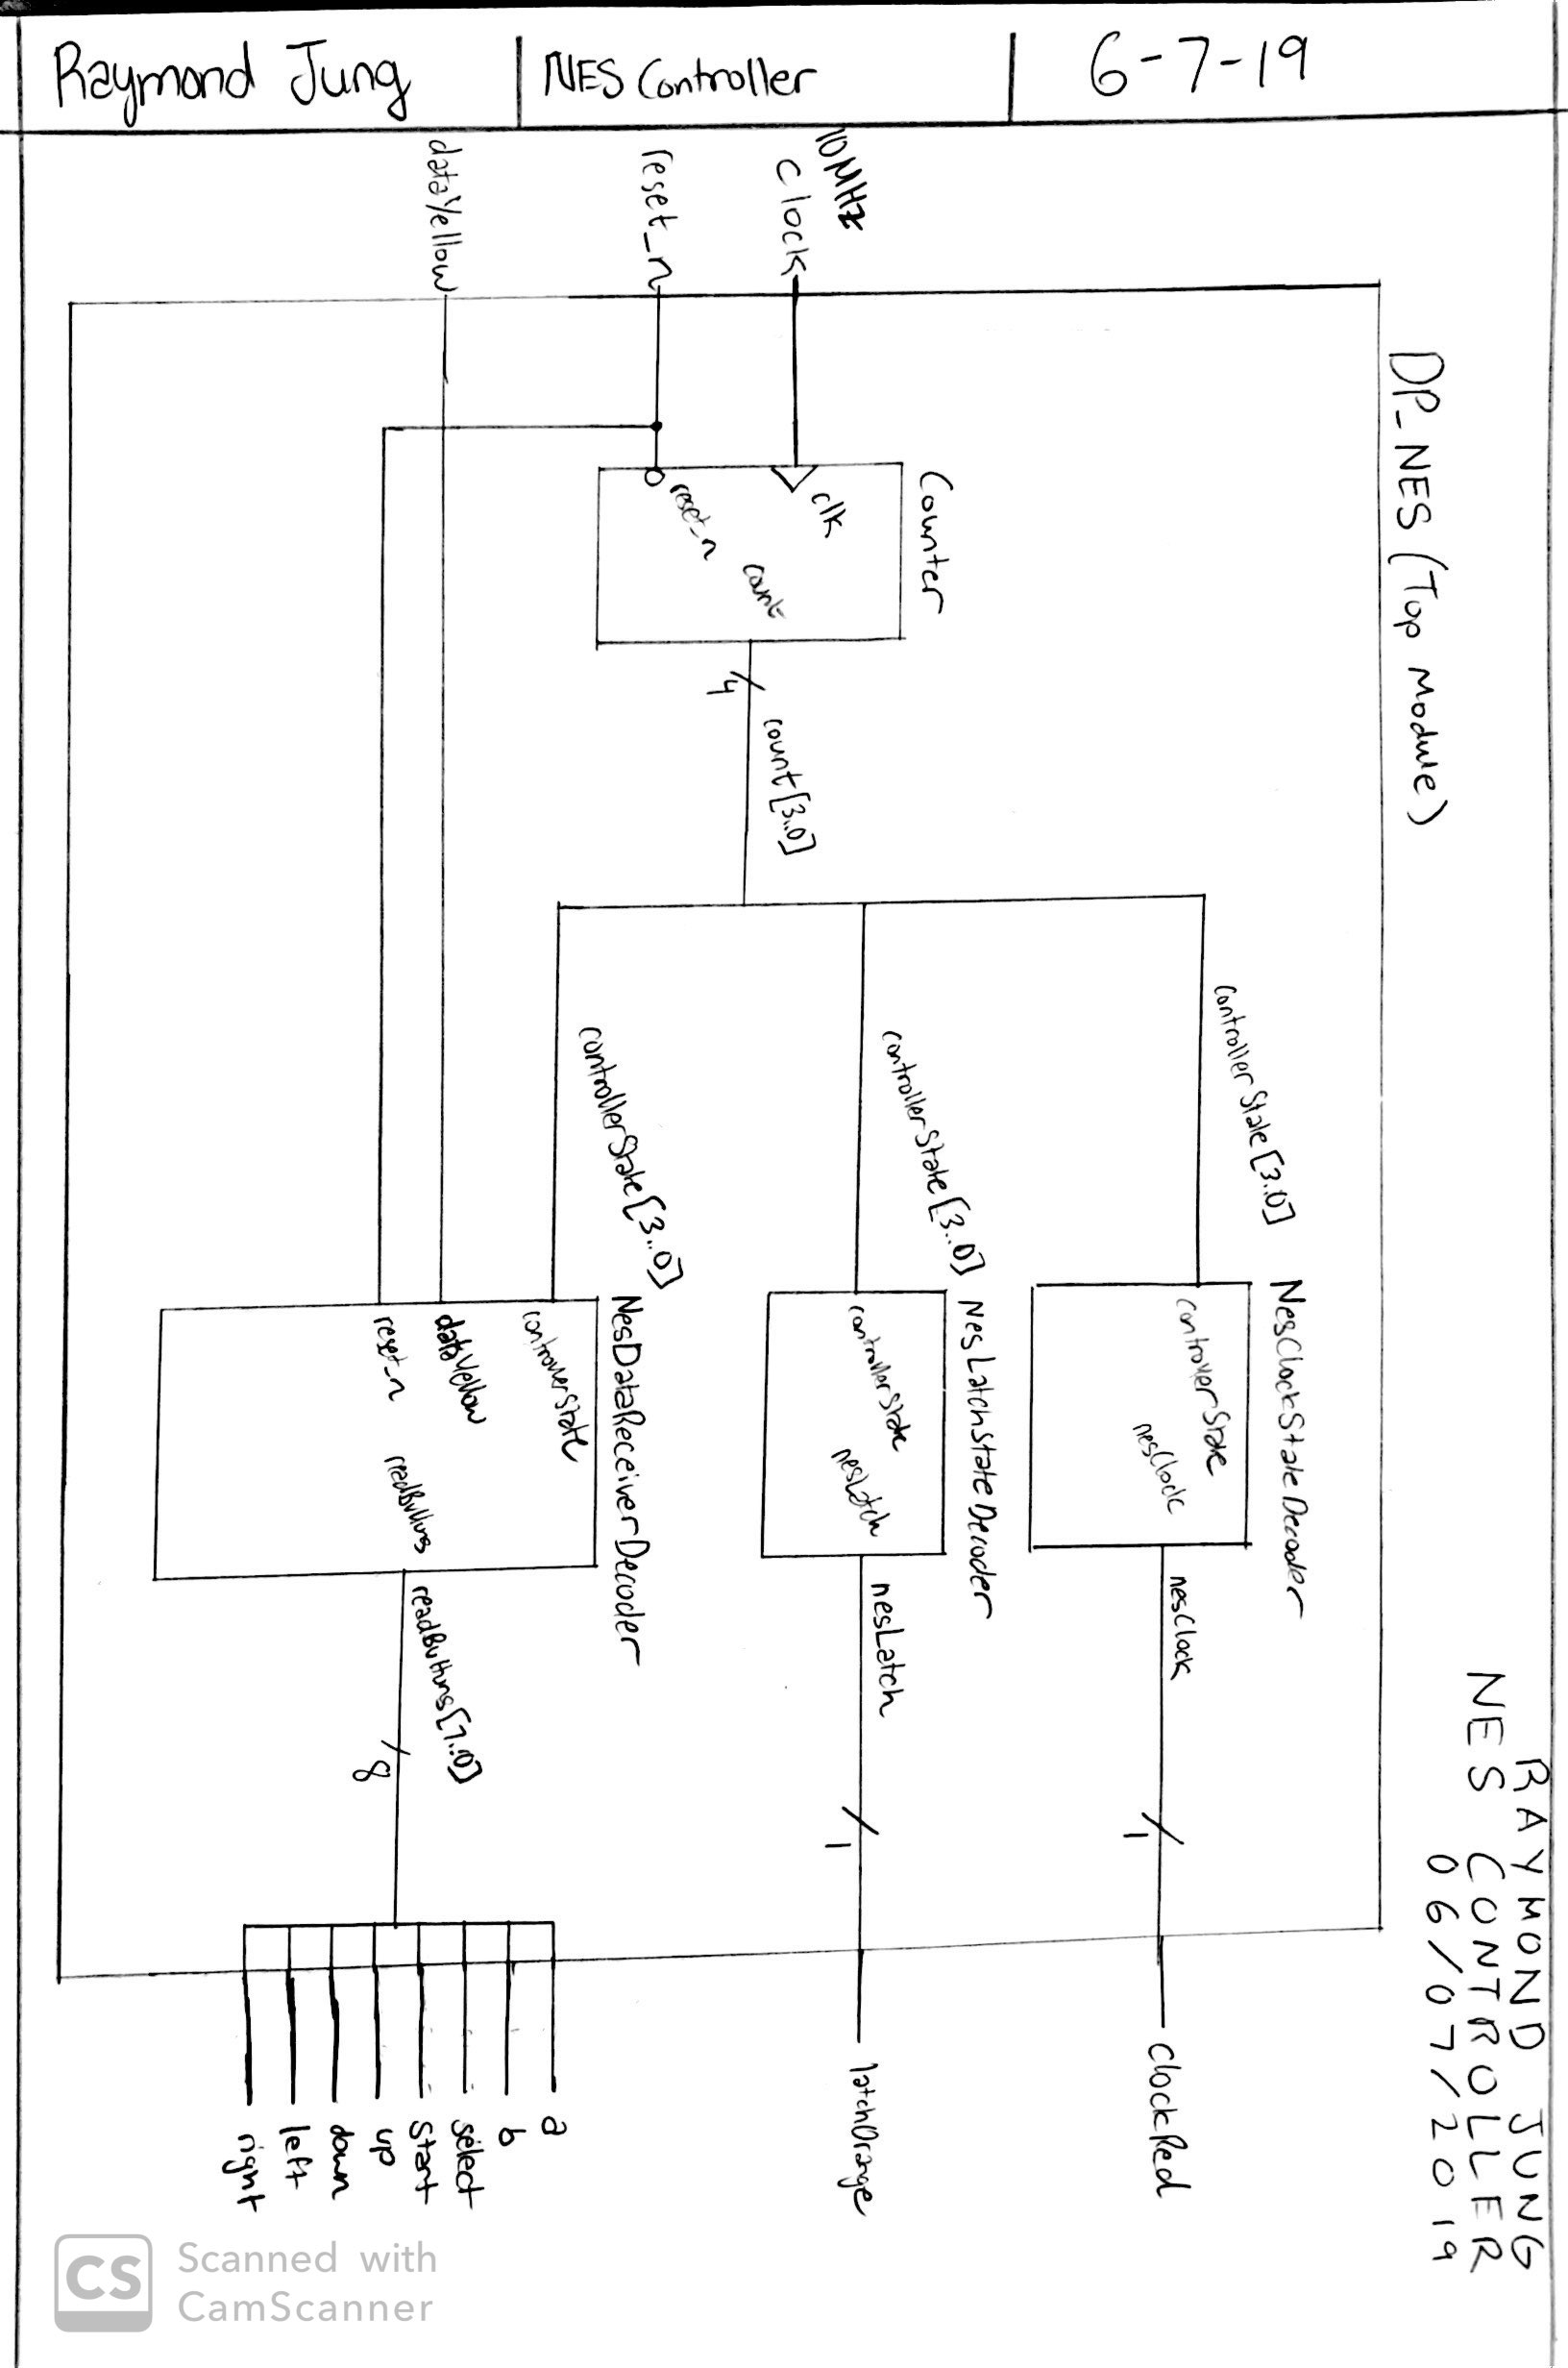
\includegraphics[width=.85\textwidth]{images/block_diagrams/nes/nestoplevel1.JPG}
	\caption{Inputs: This takes in a 1-bit dataYellow input, 10MHz clock input, and a 1-bit reset signal. \newline
	Outputs: This outputs a 1-bit clock, 1-bit latch, and a 8-bit bus that denotes the type of button being pressed \newline
	Descriptions: The NES controller takes in a clock input and as the counter within is outputting a 4-bit count to the other modules, it determines the button that is being pressed on the NES. On the FPGA, it different types of buttons are represented by the various LED segments.
	}
    \label{fig:top_level_block}
\end{figure}

\begin{figure}[H]
  \centering
    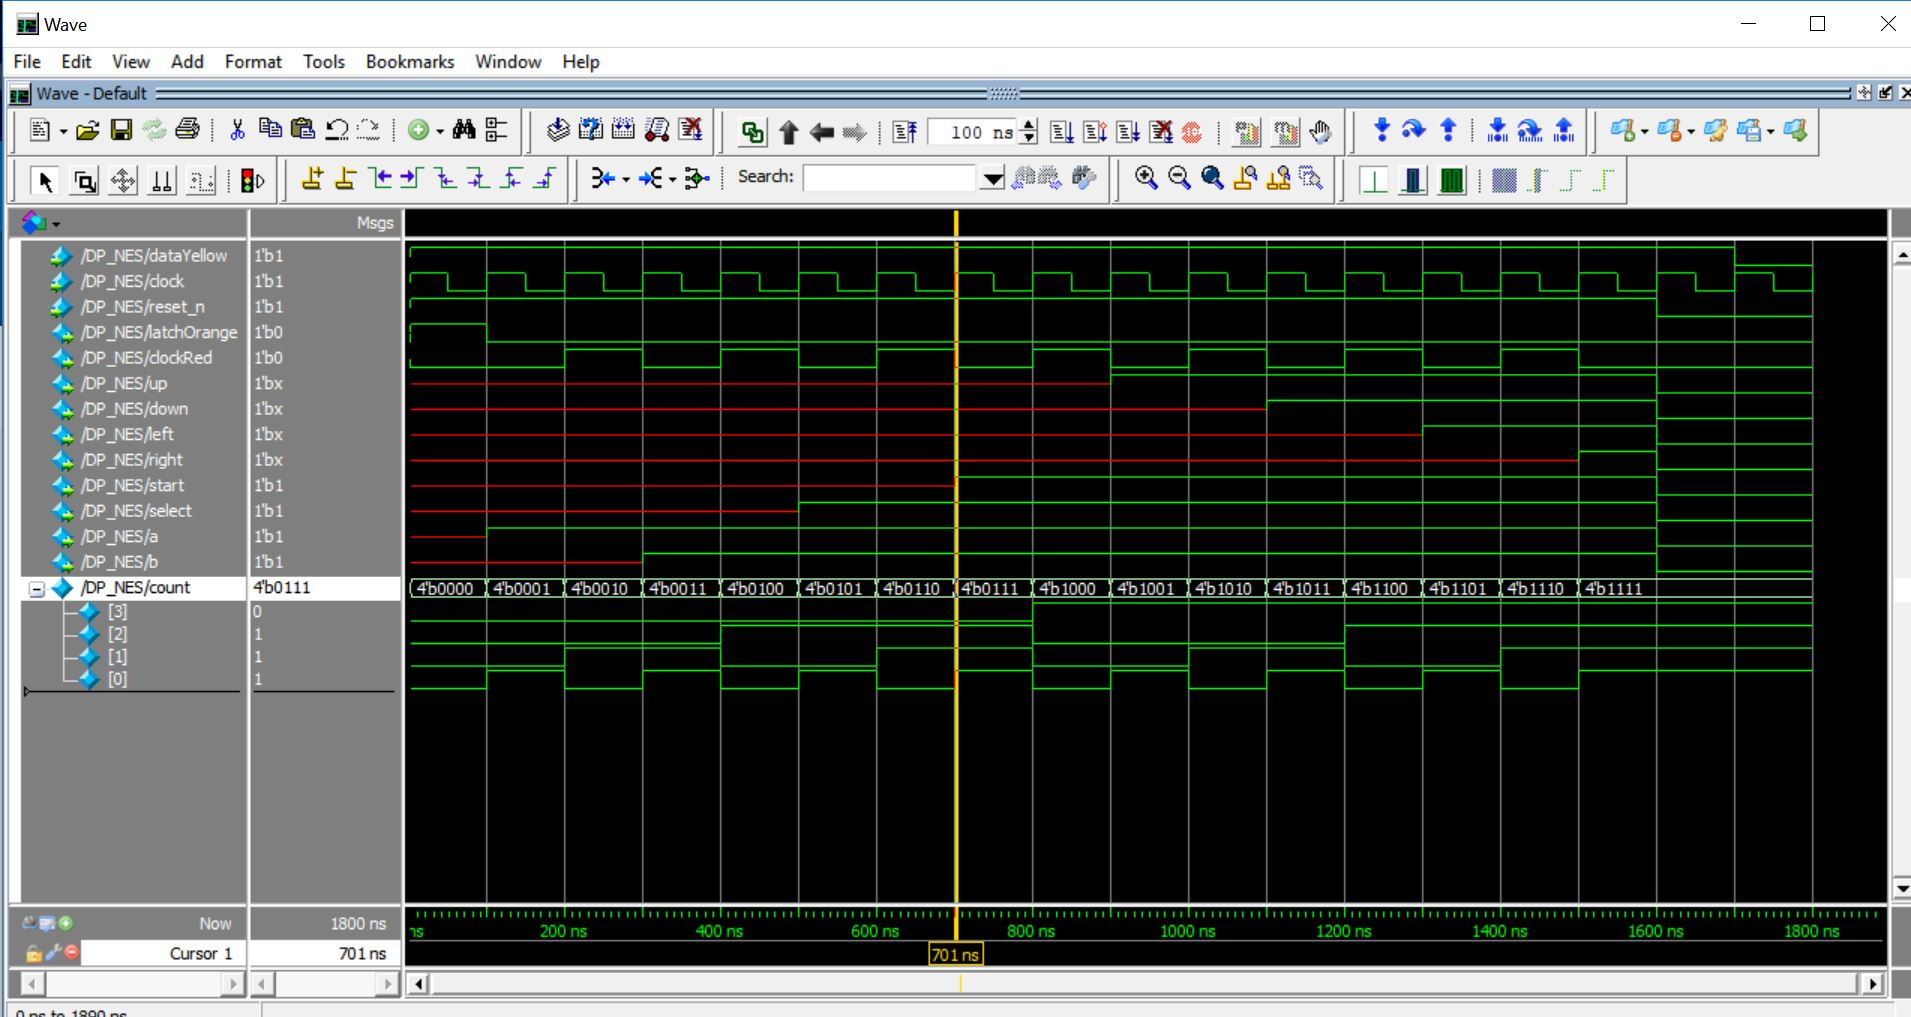
\includegraphics[width=.85\textwidth]{images/ModelSim/nesreader.JPG}
	\caption{This is the ModelSim simulated representation of the Top Level Module of the NES Controller. As one can see, as the clock input is pulsing, the reset is turned HIGH (1) and the dataYellow input is HIGH (1), the NES button outputs are each turning to a logic 1 in a period of 100ns. Meanwhile, the internal 4-bit count is incrementing from 0-F in binary. Each button on the NES turns into a logic 1 on the rising edge of the clock. As expected, once the reset is turned OFF (LOW), the functionality of the NES stops as per the 1600ns mark on the simulation.}
    \label{fig:top_level_block_sim}
\end{figure}

\subsubsection{NES Data Receiver}

\begin{figure}[H]
  \centering
    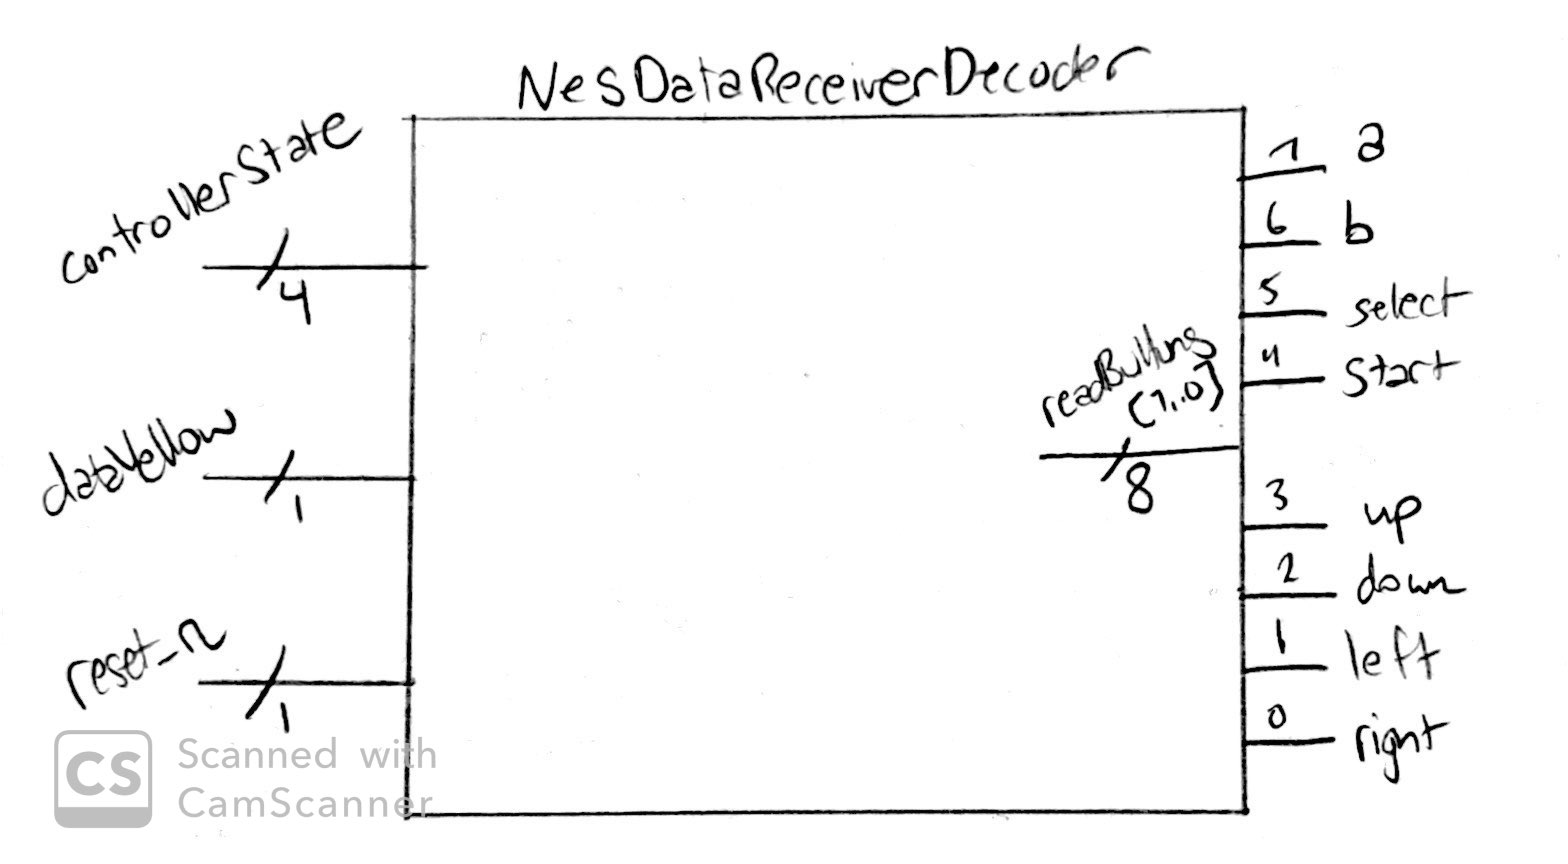
\includegraphics[width=.85\textwidth]{images/block_diagrams/nes/datareceiver2.jpg}
	\caption{Inputs: This takes in a 4-bit output from a counter, a reset signal, and a data input \newline
Outputs: The 4-bit count input goes through a decoder from within and then expands to a 8-bit output labeled right, left, down, up, start, select, b, and a. \newline
Description: This module takes in data from the counter and then highlights the buttons pressed on the the data input. It receives the data.} 
    \label{fig:data_receiver}
\end{figure}

\begin{figure}[H]
  \centering
    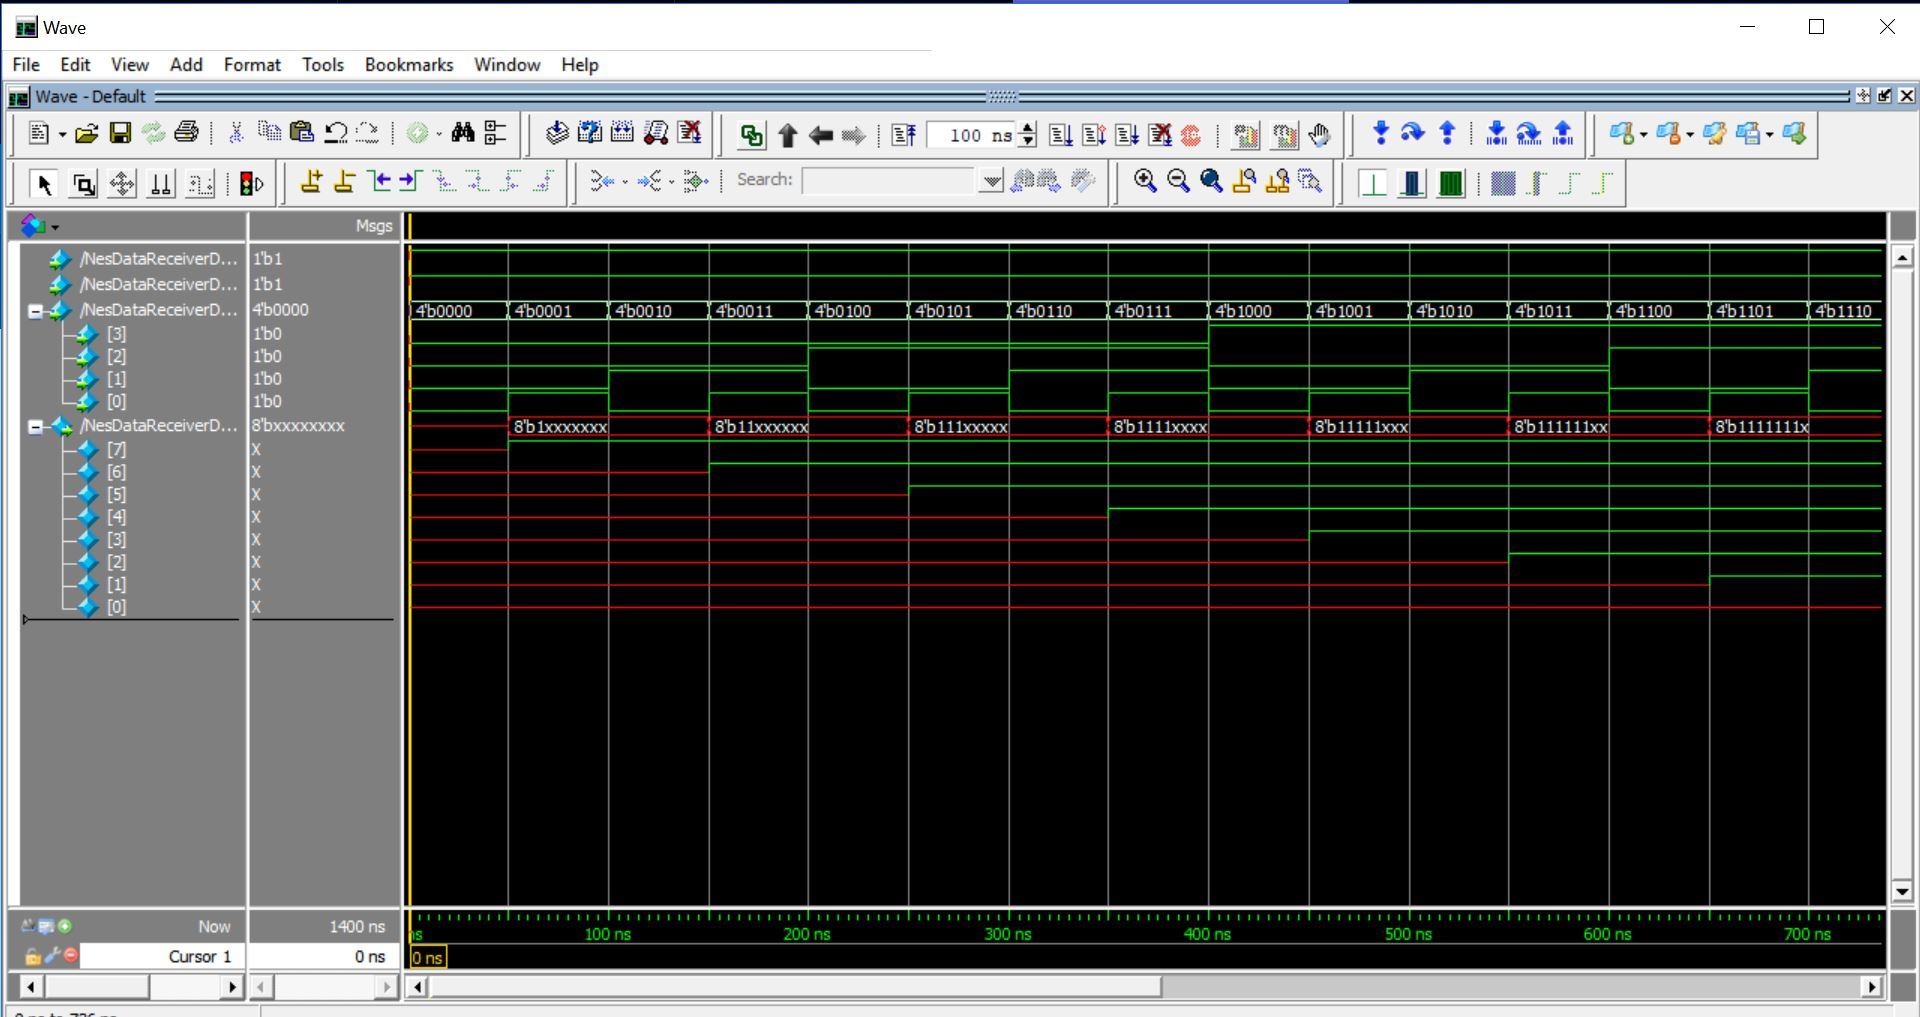
\includegraphics[width=.85\textwidth]{images/ModelSim/nesdatare.JPG}
	\caption{NES Data Receiver Simulation Part 1}
    \label{fig:data_receiver_sim}
\end{figure}

\begin{figure}[H]
  \centering
    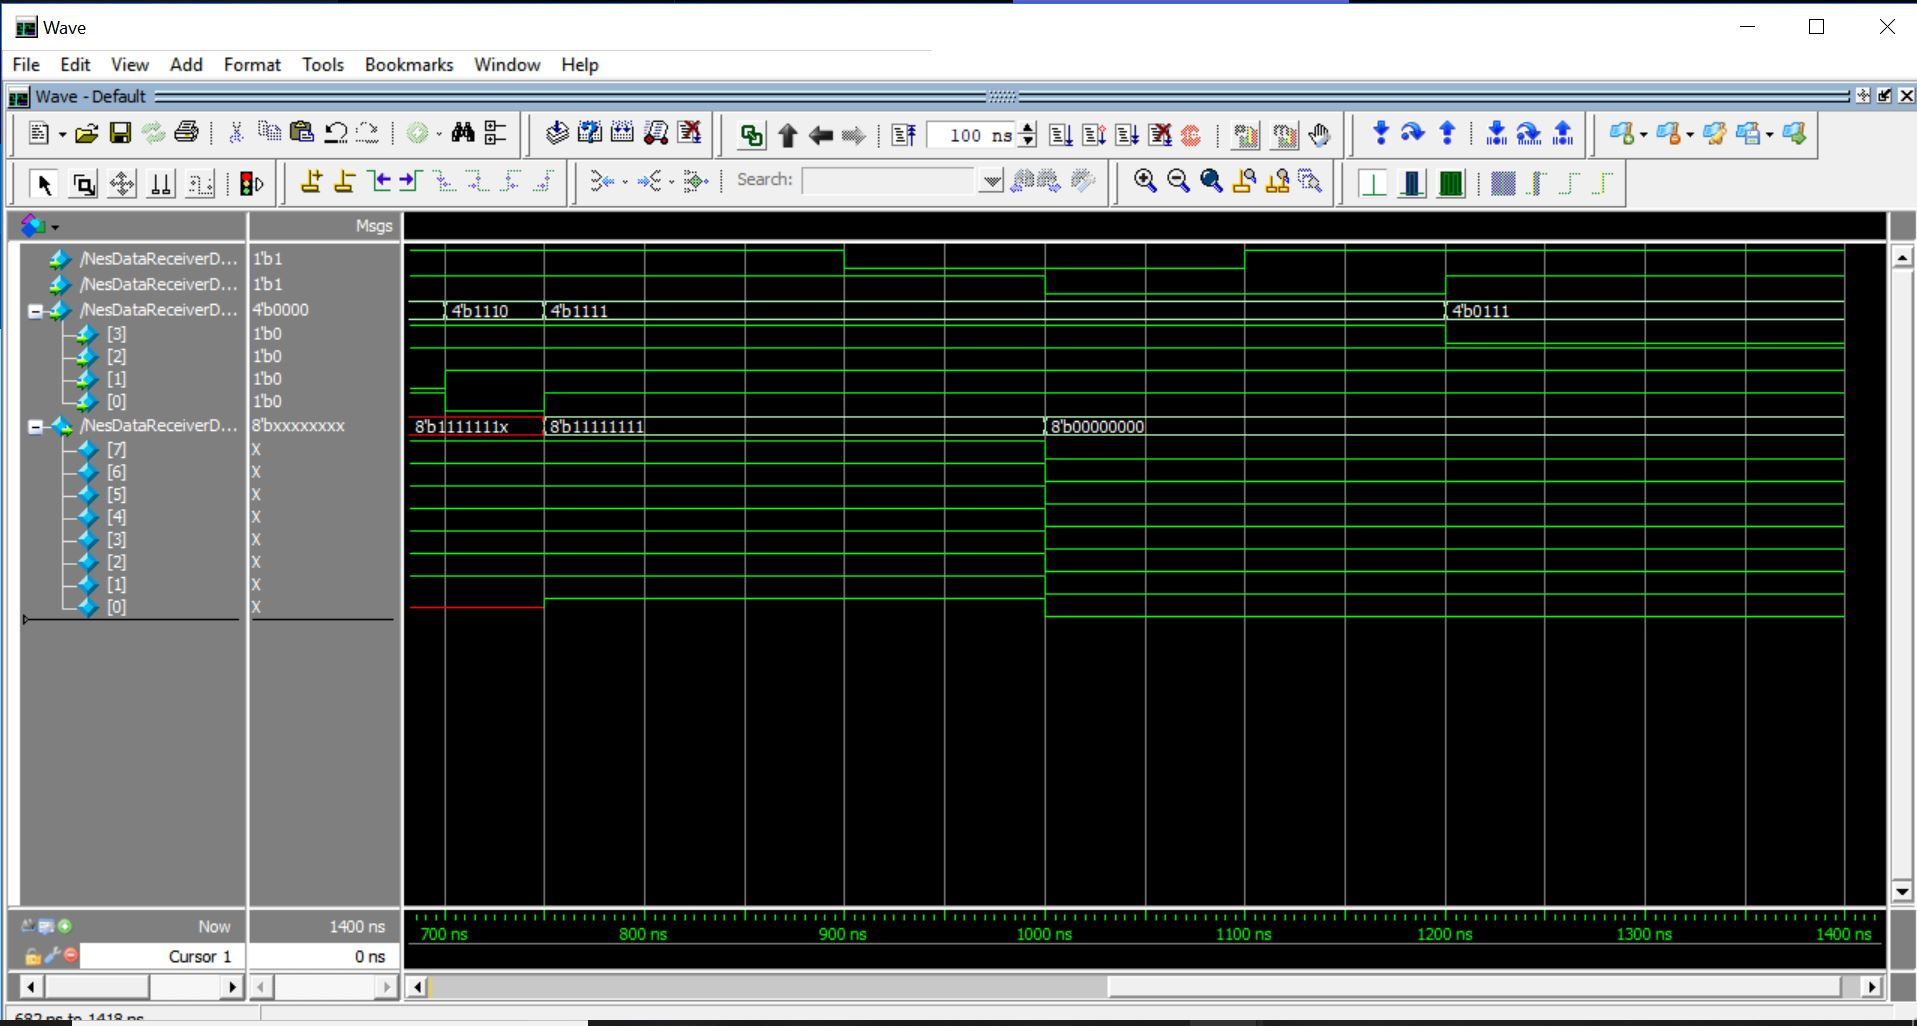
\includegraphics[width=.85\textwidth]{images/ModelSim/nesdatare2.JPG}
	\caption{This is the simulation provided for the NesDataReceiver module. In order for the NES to function, both the reset and dataYellow input have to be at a logic 1 (HIGH). As the NesDataReceiver count increments from 0->F, the output shows that the button outputs pulse to a logic 1 in increments of 100ns. Near the end of the simulation, pulling the “reset” input back to zero.}
    \label{fig:data_receiver_sim}
\end{figure}

\subsubsection{NES Latch}

\begin{figure}[H]
  \centering
    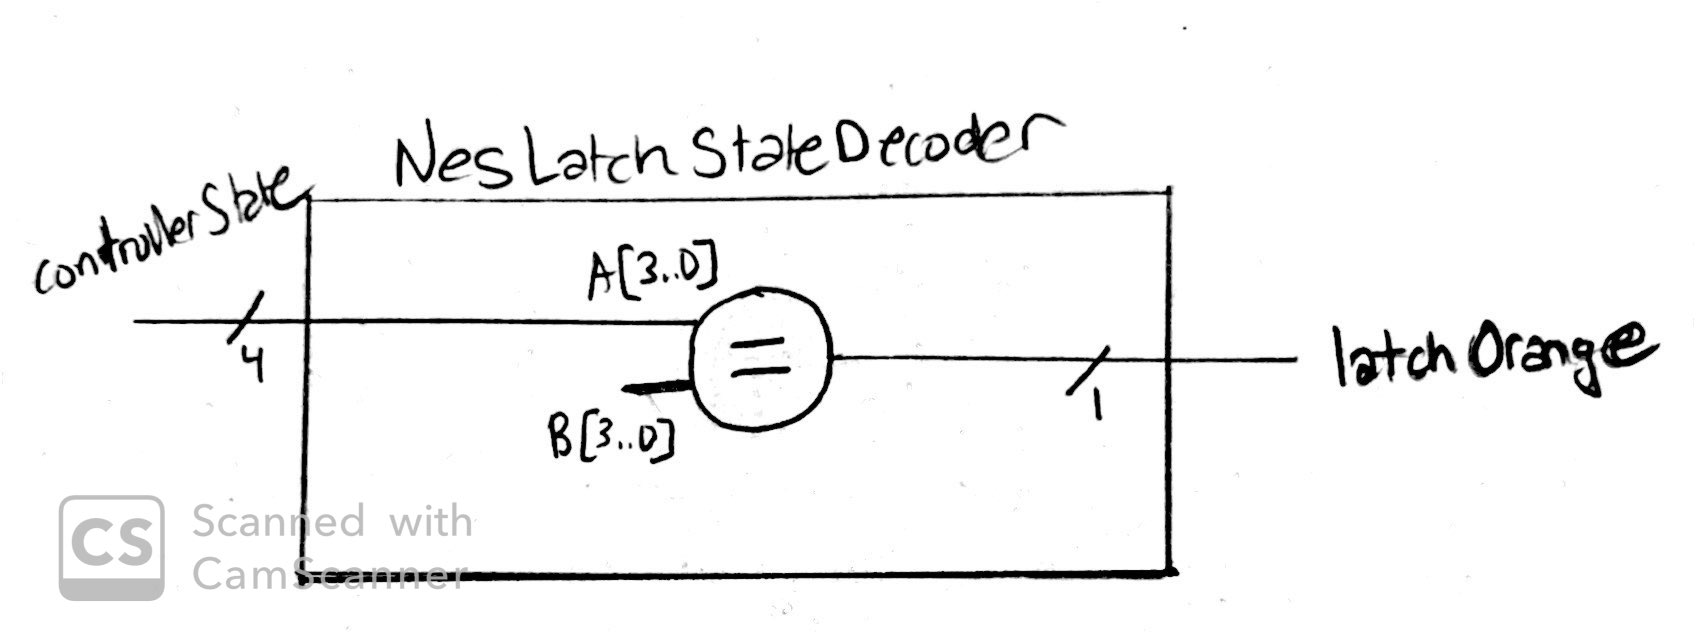
\includegraphics[width=.85\textwidth]{images/block_diagrams/nes/latch3.jpg}
	\caption{Inputs: This takes in a 4-bit output from a counter \newline
Outputs: The 4-bit count input goes through a comparator logic alongside a second 4-bit input and base the comparison value, either a 0 or 1 will be outputted. \newline
Description: This module takes in data from the counter outputs a 1-bit output labeled as “LatchOrange”}
    \label{fig:latch}
\end{figure}

\begin{figure}[H]
  \centering
    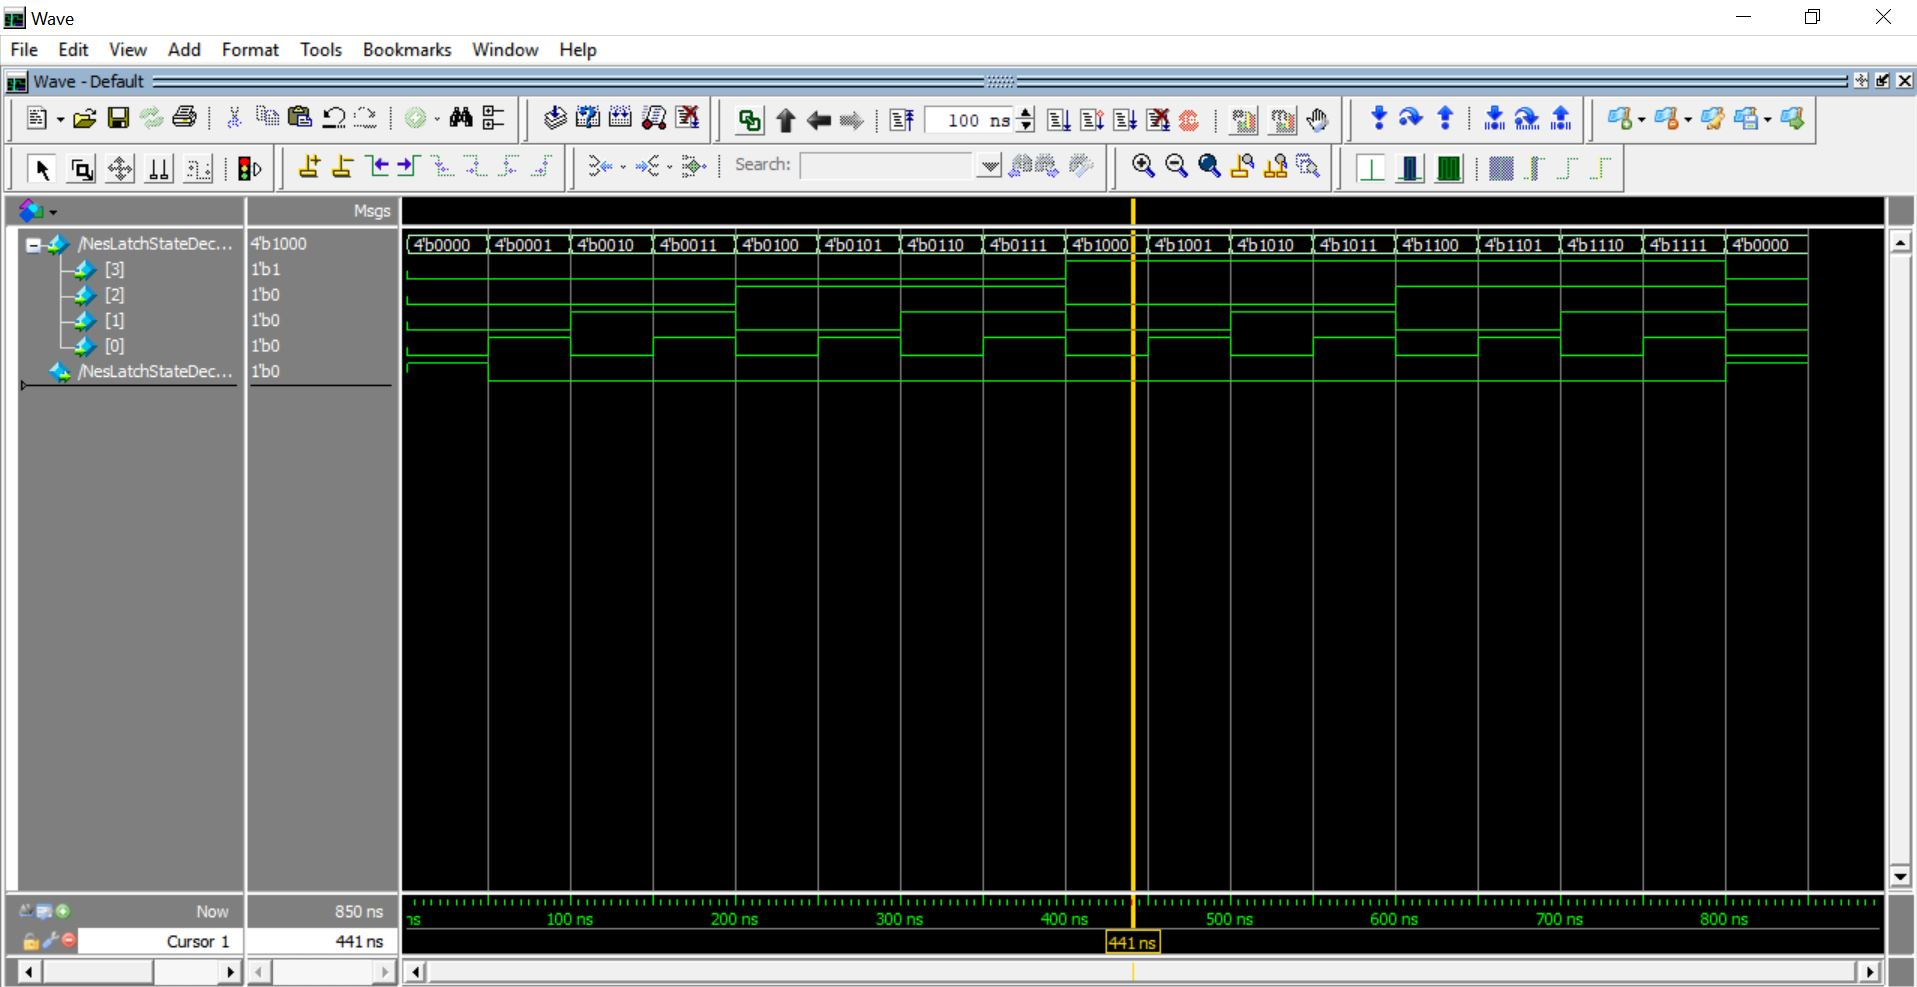
\includegraphics[width=.85\textwidth]{images/ModelSim/neslatch_sim.JPG}
	\caption{This is the individual simulation of the NesLatchStateDecoder module. As displayed, the latch state is pulled to a logic 1 when the 4-bit controllerState input is at 0. Otherwise, the output is at a logic 0. This makes sense when looking at the module, the B input is at a constant 0. As long at the 4-bit input, also named as A[3..0], is not equivalent to B (0), the latch output will always be at 0.}
    \label{fig:latch_sim}
\end{figure}

\subsubsection{NES Clock}

\begin{figure}[H]
  \centering
    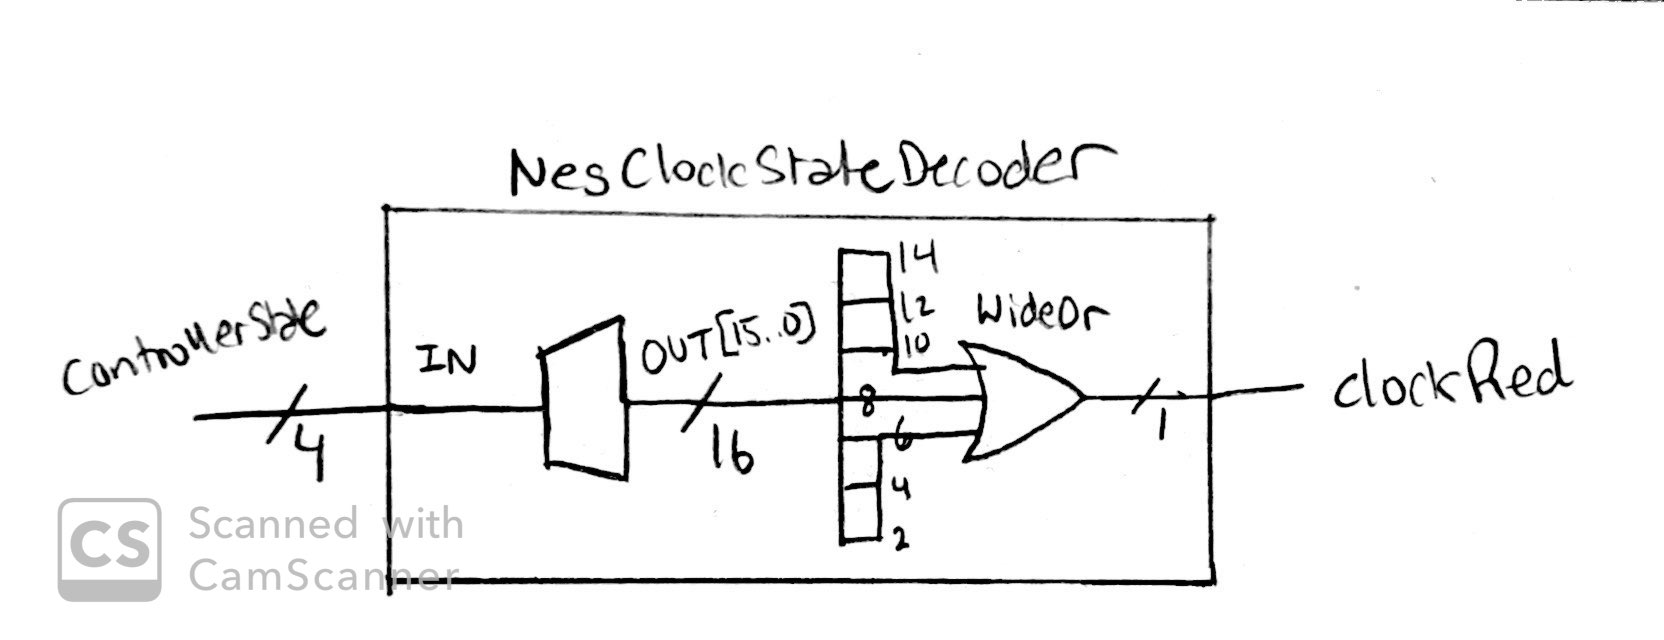
\includegraphics[width=.85\textwidth]{images/block_diagrams/nes/clock4.jpg}
	\caption{Inputs: This takes in a 4-bit output from a counter \newline
Outputs: This outputs a 1-bit clock output labeled “clockRed”
\newline
Description: This module takes in data from the counter and the decoder within expands it to a 16-bit output. It then goes through a wide OR gate that outputs a 1 if its 16-bit input is of an even value. This resembles a clock as the counter goes between odd and even values back and forth.}
    \label{fig:clock}
\end{figure}

\begin{figure}[H]
  \centering
    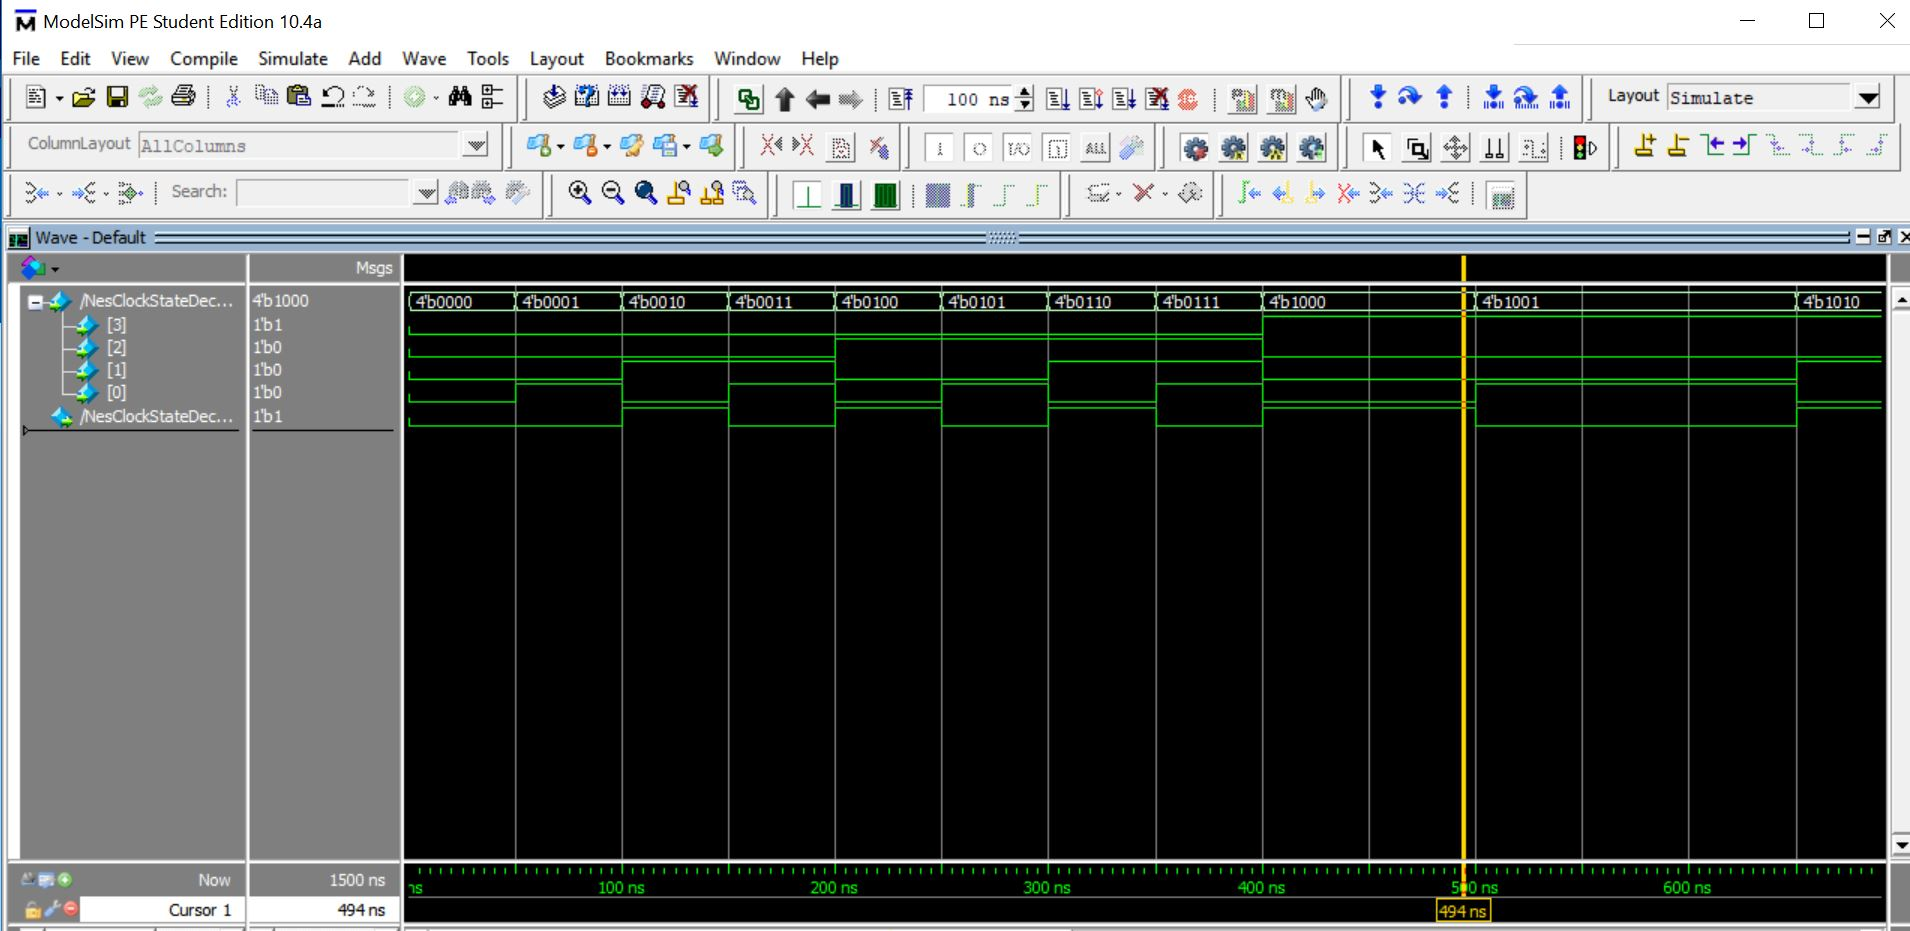
\includegraphics[width=.85\textwidth]{images/ModelSim/nesclock.JPG}
	\caption{This is the individual simulation of the NesClockStateDecoder module ran on ModelSim. As the 4-bit controllerState increments from 0->F in binary, the output is shown to be operating as it should with a clock pulsing between equal intervals. Looking more in depth at the NesClockStateDecoder, the OR gate implemented only outputs a 1 on even inputs. Looking at the simulation here, one can see that the output is at a logic 1 for every even number input shown in binary such as 4’b0010 and 4’0101.}
    \label{fig:clock_sim}
\end{figure}

\subsubsection{NES Counter}

\begin{figure}[H]
  \centering
    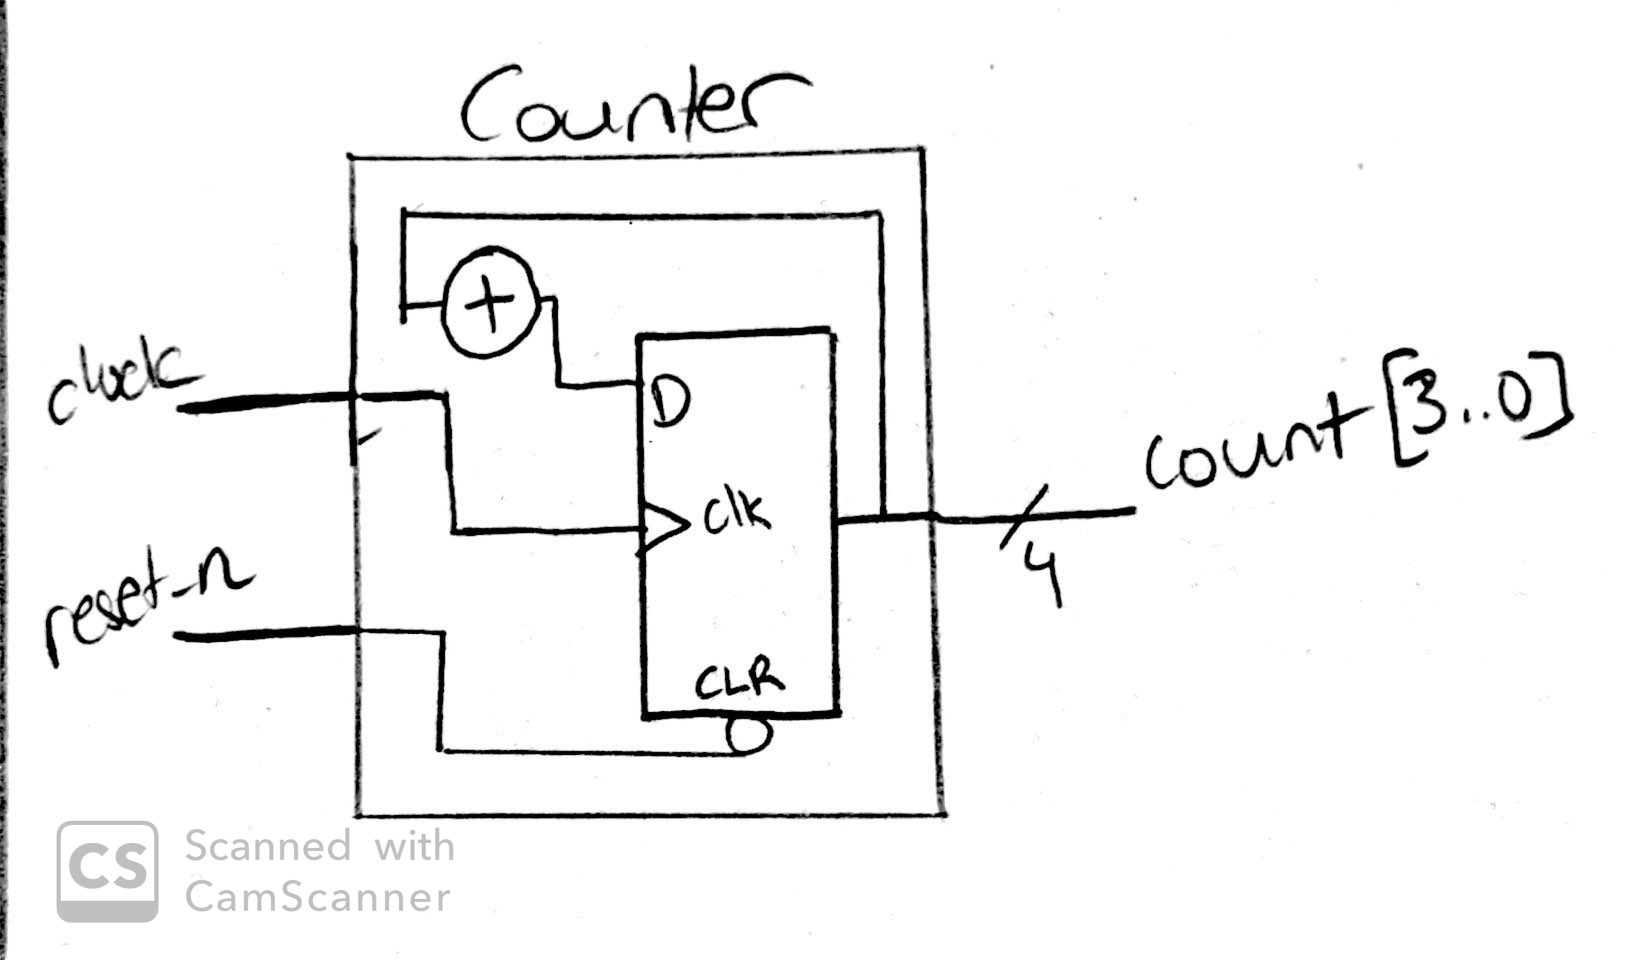
\includegraphics[width=.85\textwidth]{images/block_diagrams/nes/counter5.jpg}
	\caption{Inputs: This takes in a 10MHz clock input and a reset signal \newline
Outputs: This outputs a 4-bit count \newline
Description: As the reset signal is a logic HIGH (1) and there is a clock input running through the counter, the counter will continue to increment starting from 0 to F and then back around. Upon a reset signal that’s turned LOW, the counter will reset to 0.}
    \label{fig:counter}
\end{figure}

\begin{figure}[H]
  \centering
    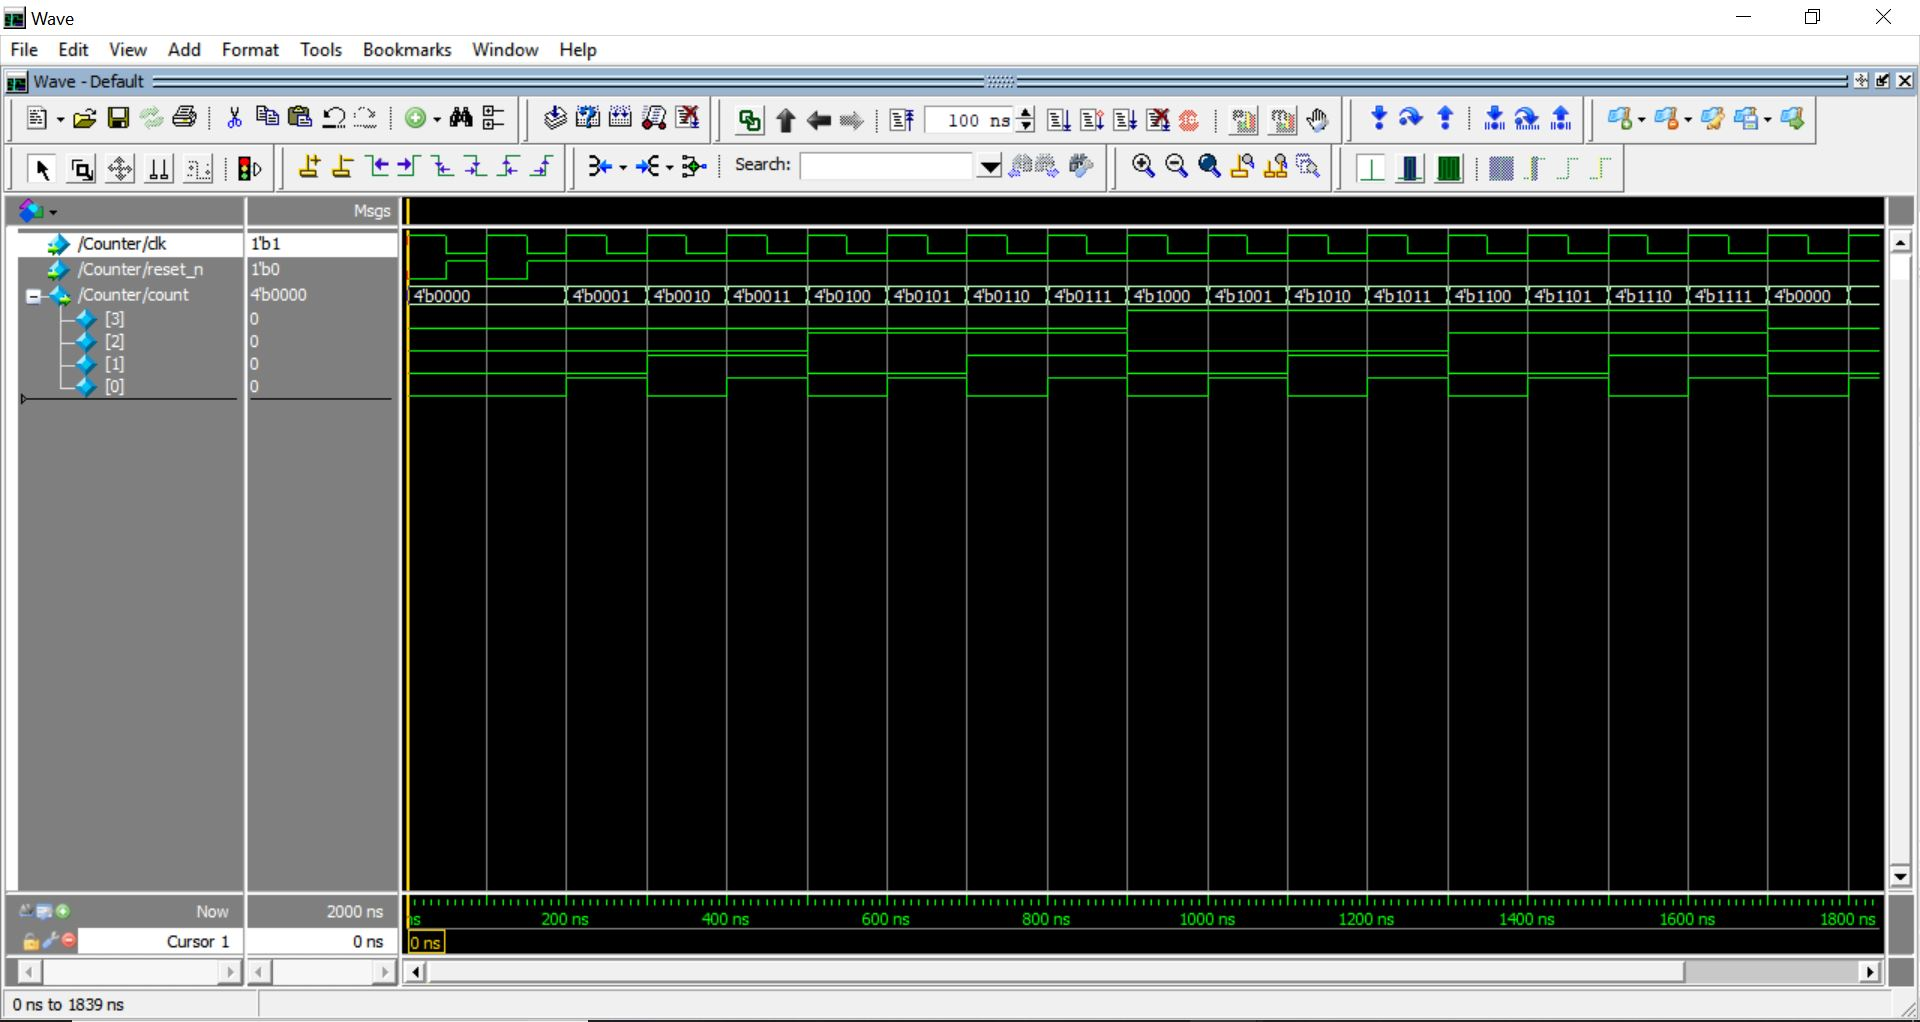
\includegraphics[width=.85\textwidth]{images/ModelSim/nescounter.JPG}
	\caption{This simulation is representing the individual counter module of the NES controller. By sending in a clock input at the start and testing the reset input, one can see that the counter doesn’t operate when reset is LOW (expected). As reset shifts to a logic 1 upon 150ns and stays at 1, the counter is shown to be functioning. It is incrementing by 1 from 0->F (represented in binary), and once it reaches F, the next value for the output returns to 0.}
    \label{fig:counter_sim}
\end{figure}

\subsection{PS2 Keyboard Decoder}

\begin{figure}[H]
  \centering
    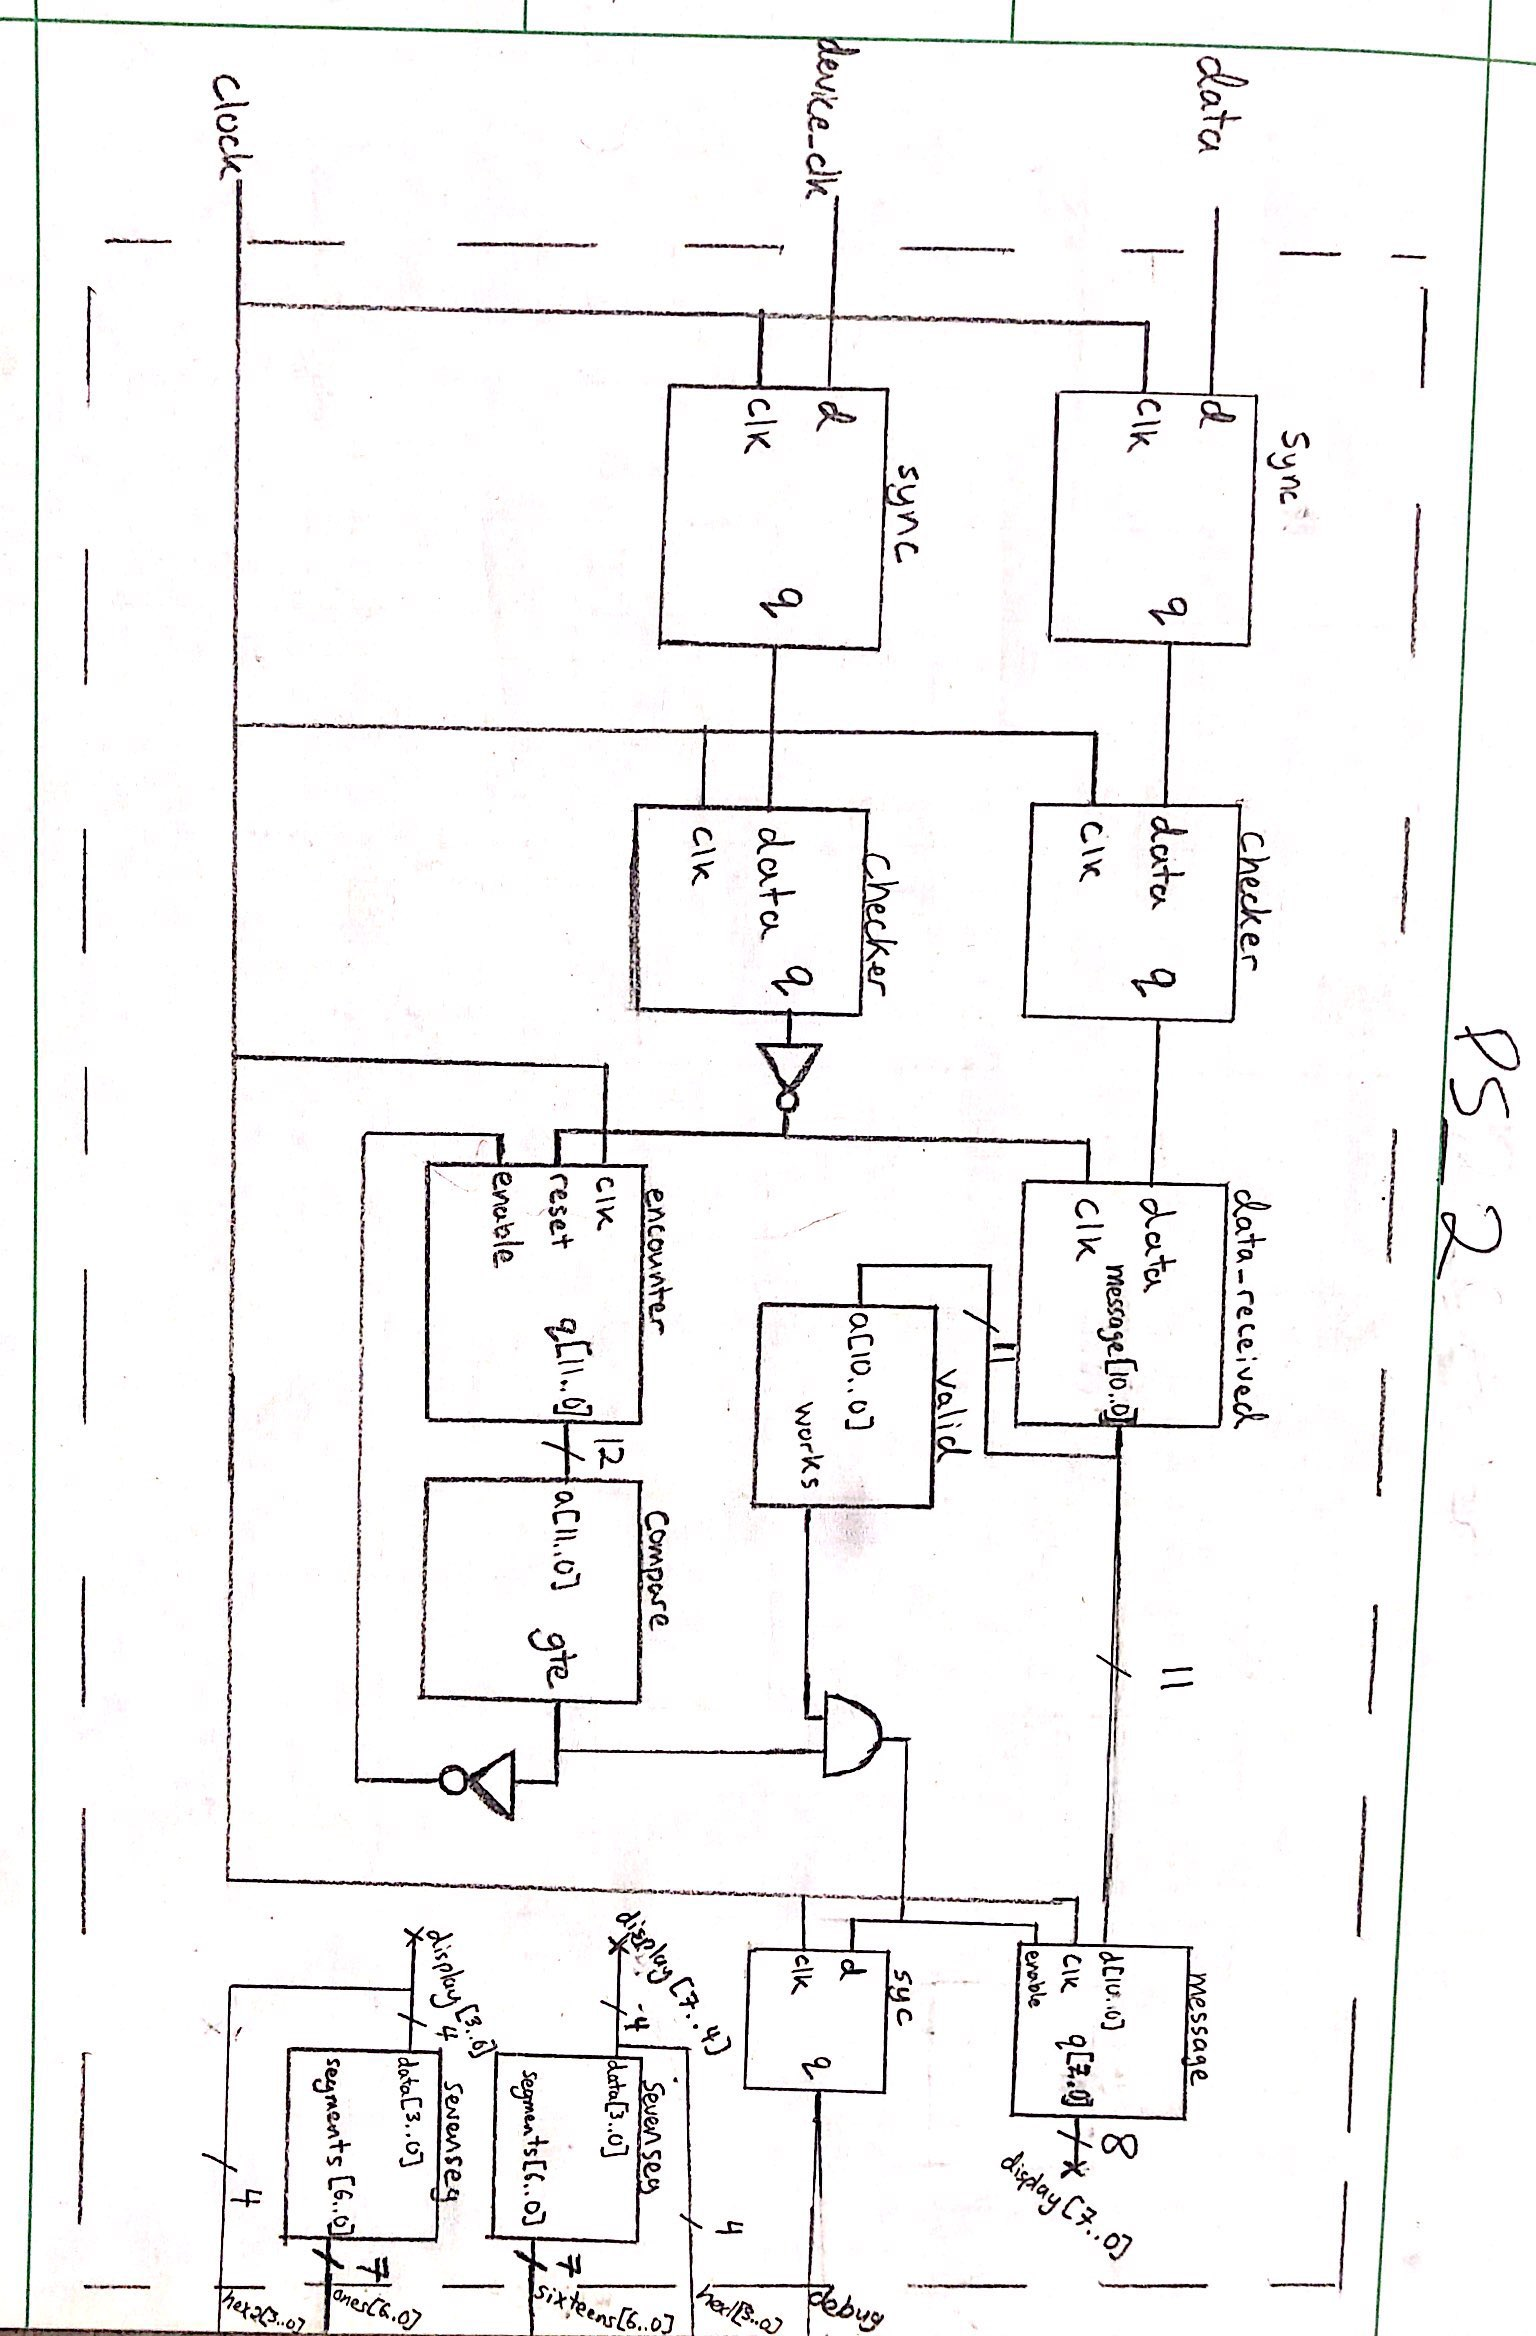
\includegraphics[width=0.6\textwidth,angle=90,origin=c]{images/block_diagrams/PS2/PS2Top.jpg}
	\caption{Inputs: This takes in a 10-12.6kHz clock, 10MHz clock, and a 1-bit data signal. \newline
	Outputs: This outputs a 1-bit debug, two 4-bit buses with the hex values of the button pressed, and two 7-bit buses that are meant to drive  an active-low seven segment display. \newline}
	\label{fig:PS2_decoder}
\end{figure}

\subsubsection{Simulation of top level}

\begin{figure}[H]
  \centering
    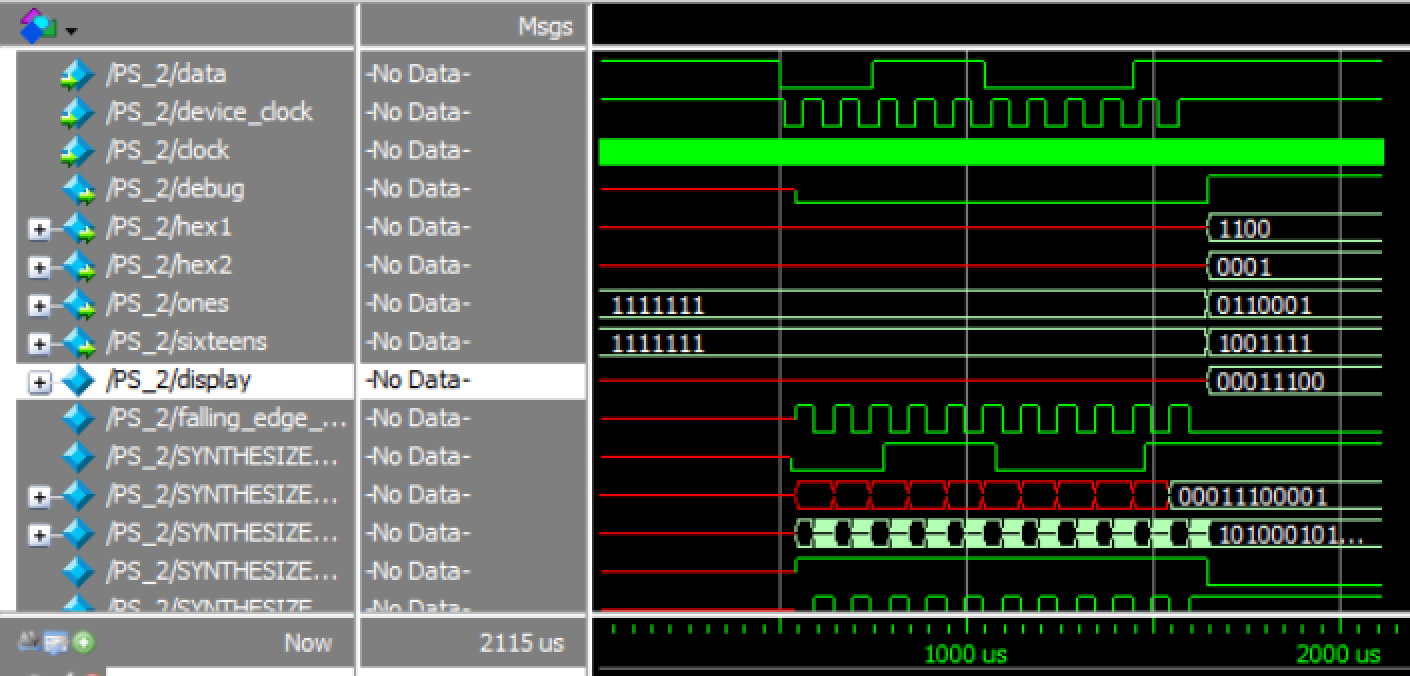
\includegraphics[width=0.6\textwidth]{images/ModelSim/PS2/PS2_Controller.png}
	\caption{Above is the ModelSim simulation of the top level PS2 driver for the FPGA. In this diagram, the clock represents the 50MHz clock on the FPGA}
	\label{fig:PS2_topsim}
\end{figure}
\subsubsection{Next Individual Block}
\subsubsection{Next Individual Block}
\subsubsection{Next Individual Block}
\subsubsection{Next Individual Block}

\subsection{VCR Remote Decoder}

\textbf{Input:} This module reads a 50MHz clock signal (\code{i_clk}), an active low reset (\code{i_reset_n}), and a signal from an IR sensor (\code{i_ir_signal}).
\\ \\
\textbf{Output:} \code{o_button_ss[6..0]} is used to display the latest VCR remote button value received on a 7-segment display.  This output also turns the display off if no code has yet been recieved or an unrecognized code was received.  \code{o_checksum_valid} indicates whether the latest 32-bit code received has a vaild checksum, which is be the case for all valid codes.
\\ \\
The code for this block is given in \autoref{lst:sv_vcr_ir_decoder}.

\begin{figure}[H]
	\centering
	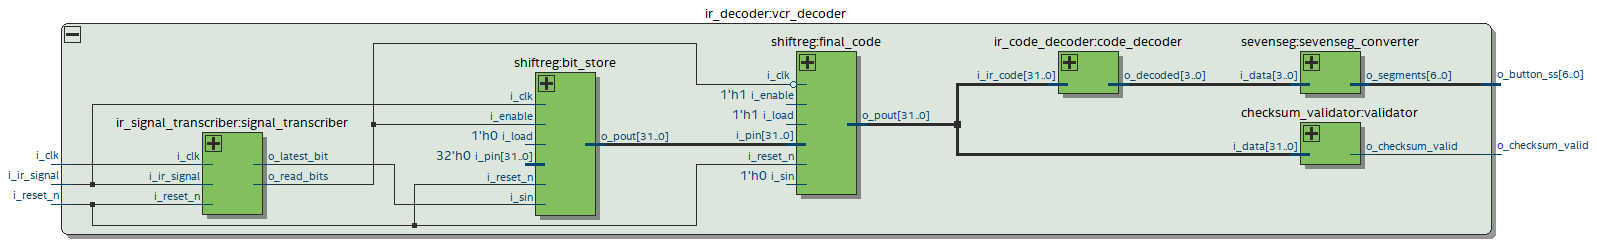
\includegraphics[width=0.85\textwidth]{images/block_diagrams/vcr_remote/ir_decoder.png}
	\caption{An expanded view of the top-level VCR remote decoder block in \autoref{fig:top_level}.  This interprets codes sent over IR using the NEC protocol as described in \cite{nec}.  A signal transcriber (\code{signal_transcriber}) determines whether bits are currently being sent and the most recent bit.  These are fed into a shift register (\code{bit_store}) at the end of the transmission of each bit.  Once an entire code has been transmitted, the contents of that register are transferred to another, \code{final_code}.  The checksum of this code is then checked by the checksum validator \code{validator} and output to \code{o_checksum_valid}.  It is also decoded to the number pressed on the remote by a decoder (\code{code_decoder}) and then converted to a 7-segment display signal by \code{segsev_converter} before being output to \code{o_button_ss}.}
	\label{fig:block_vcr_ir_decoder}
\end{figure}

\begin{figure}[H]
	\centering
	\includegraphics[width=.8\textwidth]{images/sim/vcr_remote/0.png}
	\caption{Simulation results for a "0" signal (see \autoref{lst:sim_vcr_ir_decoder_0} for simulation code).}
\end{figure}

\begin{figure}[H]
	\centering
	\includegraphics[width=.8\textwidth]{images/sim/vcr_remote/1.png}
	\caption{Simulation results for a "1" signal (see \autoref{lst:sim_vcr_ir_decoder_1} for simulation code).}
\end{figure}

\begin{figure}[H]
	\centering
	\includegraphics[width=.8\textwidth]{images/sim/vcr_remote/2.png}
	\caption{Simulation results for a "2" signal (see \autoref{lst:sim_vcr_ir_decoder_2} for simulation code).}
\end{figure}

\begin{figure}[H]
	\centering
	\includegraphics[width=.8\textwidth]{images/sim/vcr_remote/3.png}
	\caption{Simulation results for a "3" signal (see \autoref{lst:sim_vcr_ir_decoder_3} for simulation code).}
\end{figure}

\begin{figure}[H]
	\centering
	\includegraphics[width=.8\textwidth]{images/sim/vcr_remote/4.png}
	\caption{Simulation results for a "4" signal (see \autoref{lst:sim_vcr_ir_decoder_4} for simulation code).}
\end{figure}

\begin{figure}[H]
	\centering
	\includegraphics[width=.8\textwidth]{images/sim/vcr_remote/5.png}
	\caption{Simulation results for a "5" signal (see \autoref{lst:sim_vcr_ir_decoder_5} for simulation code).}
\end{figure}

\begin{figure}[H]
	\centering
	\includegraphics[width=.8\textwidth]{images/sim/vcr_remote/6.png}
	\caption{Simulation results for a "6" signal (see \autoref{lst:sim_vcr_ir_decoder_6} for simulation code).}
\end{figure}

\begin{figure}[H]
	\centering
	\includegraphics[width=.8\textwidth]{images/sim/vcr_remote/7.png}
	\caption{Simulation results for a "7" signal (see \autoref{lst:sim_vcr_ir_decoder_7} for simulation code).}
\end{figure}

\begin{figure}[H]
	\centering
	\includegraphics[width=.8\textwidth]{images/sim/vcr_remote/8.png}
	\caption{Simulation results for a "8" signal (see \autoref{lst:sim_vcr_ir_decoder_8} for simulation code).}
\end{figure}

\begin{figure}[H]
	\centering
	\includegraphics[width=.8\textwidth]{images/sim/vcr_remote/9.png}
	\caption{Simulation results for a "9" signal (see \autoref{lst:sim_vcr_ir_decoder_9} for simulation code).}
\end{figure}

\begin{figure}[H]
	\centering
	\includegraphics[width=.8\textwidth]{images/sim/vcr_remote/sequence.png}
	\caption{Simulation results for a "1" signal followed by a "2" signal (see \autoref{lst:sim_vcr_ir_decoder_sequence} for simulation code).}
\end{figure}

\begin{figure}[H]
	\centering
	\includegraphics[width=.8\textwidth]{images/sim/vcr_remote/bad_checksum.png}
	\caption{Simulation results for a signal producing an invalid code (see \autoref{lst:sim_vcr_ir_decoder_bad_checksum} for simulation code).}
\end{figure}

\subsubsection{IR Signal Transcriber}

\textbf{Input:} This module reads a 50MHz clock signal (\code{i_clk}), an active low reset (\code{i_reset_n}), and a signal from an IR sensor (\code{i_ir_signal}).
\\ \\
\textbf{Output:} \code{o_latest_bit} indicates the last bit seen in the IR signal.  \code{o_read_bits} indicates whether new bits are currently being read.
\\ \\
The code for this block is given in \autoref{lst:sv_vcr_ir_signal_transcriber}.
\\ \\
The simulations in the previous section also serve to simulate this module.

\begin{figure}[H]
	\centering
	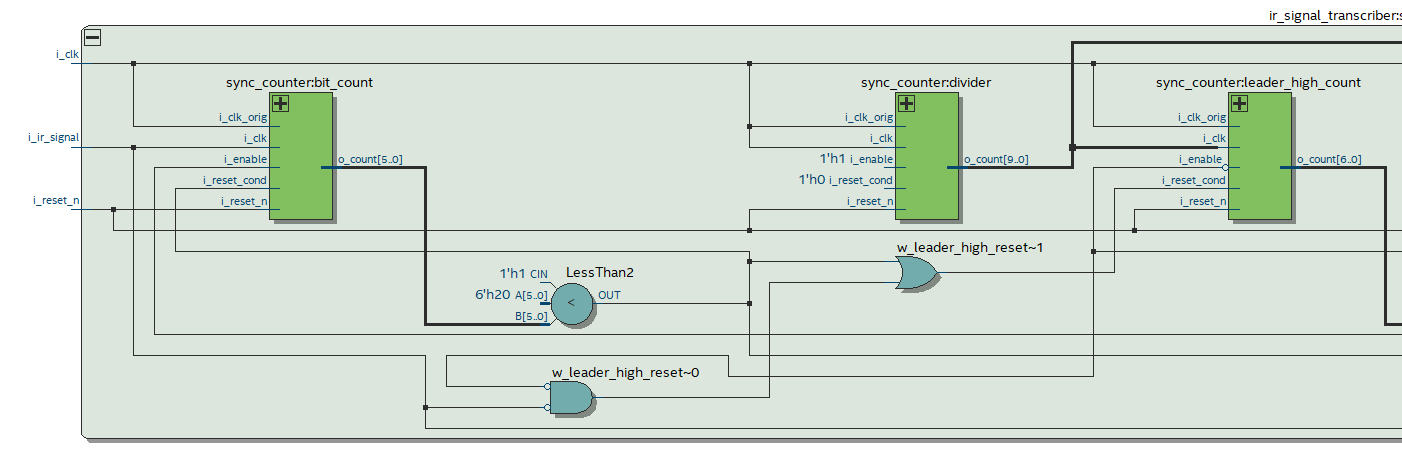
\includegraphics[width=.85\textwidth]{images/block_diagrams/vcr_remote/ir_signal_transcriber_1.png}
	\caption{An expanded view of the first half of the IR signal transcriber block in \autoref{fig:block_vcr_ir_decoder}.  A 10-bit counter (\code{divider}) divides the 10MHz input clock down to 10KHz.  Another counter, \code{leader_high_count}, uses this clock to count up as long as the input signal is high (for the high part of the leader) and it hasn't reached the length of that high part.  It resets if the signal goes low again before it has reached that value and when 32 bits have been read.  The bit counter to the left is enabled when the entire leader has ended and increments for each bit read.  It also resets when 32 bits have been read.}
	\label{fig:block_vcr_ir_signal_transcriber_1}
\end{figure}

\begin{figure}[H]
	\centering
	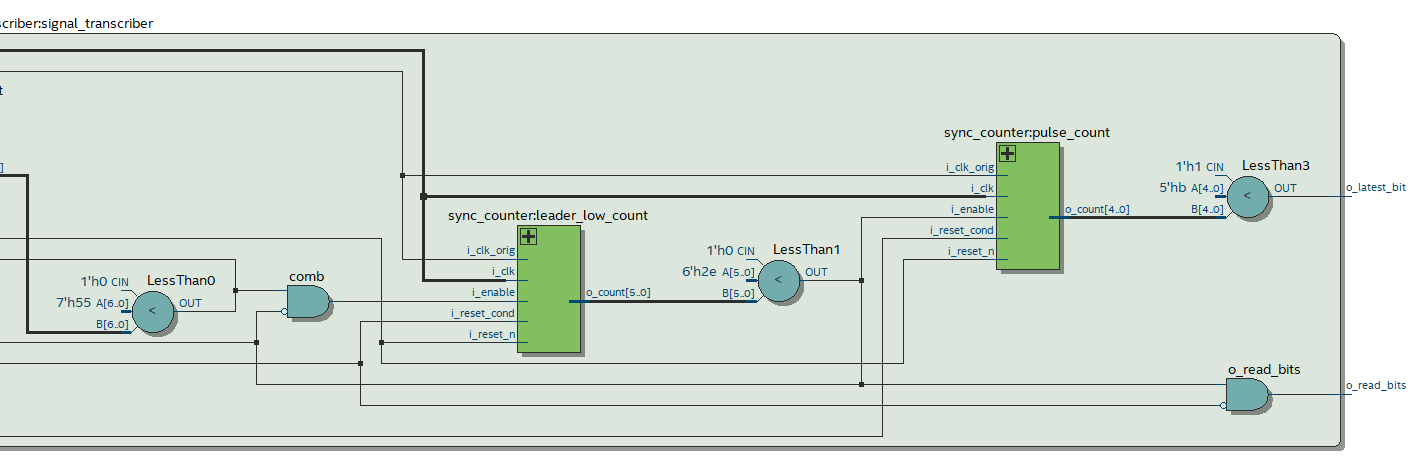
\includegraphics[width=.85\textwidth]{images/block_diagrams/vcr_remote/ir_signal_transcriber_2.png}
	\caption{An expanded view of the second half of the IR signal transcriber block in \autoref{fig:block_vcr_ir_decoder}.  A counter (\code{leader_low_count}) acts similarly to \code{leader_high_count}.  It is enabled when the high part of the leader has ended and counts up to the length of the low part of the leader.  It resets once it has reached that length.  At this point, \code{pulse_count} is enabled and counts as long as the signal is low.  This is used to determine the length of each pulse distance.  A comparator determines if the distance is less than a cutoff (a 0) or greater than the cutoff (signifying  a 1).  Additionally, \code{o_read_bits} is set high when the low part of the leader has ended and fewer than 32 bits have been read.}
	\label{fig:block_vcr_ir_signal_transcriber_2}
\end{figure}

\subsubsection{Sync-Counter}

\textbf{Input:} This module reads a clock signal (\code{i_clk}), a separate synchronizer clock signal (\code{i_clk_orig}), an enable signal (\code{i_enable}), and an active low reset (\code{i_reset_n}).  It also takes in another reset input (\code{i_reset_cond}) that is active high and also resets the counter.
\\ \\
\textbf{Output:} \code{o_count} provides the current value of the counter.
\\ \\
The code for this block is given in \autoref{lst:sv_vcr_sync_counter}.

\begin{figure}[H]
	\centering
	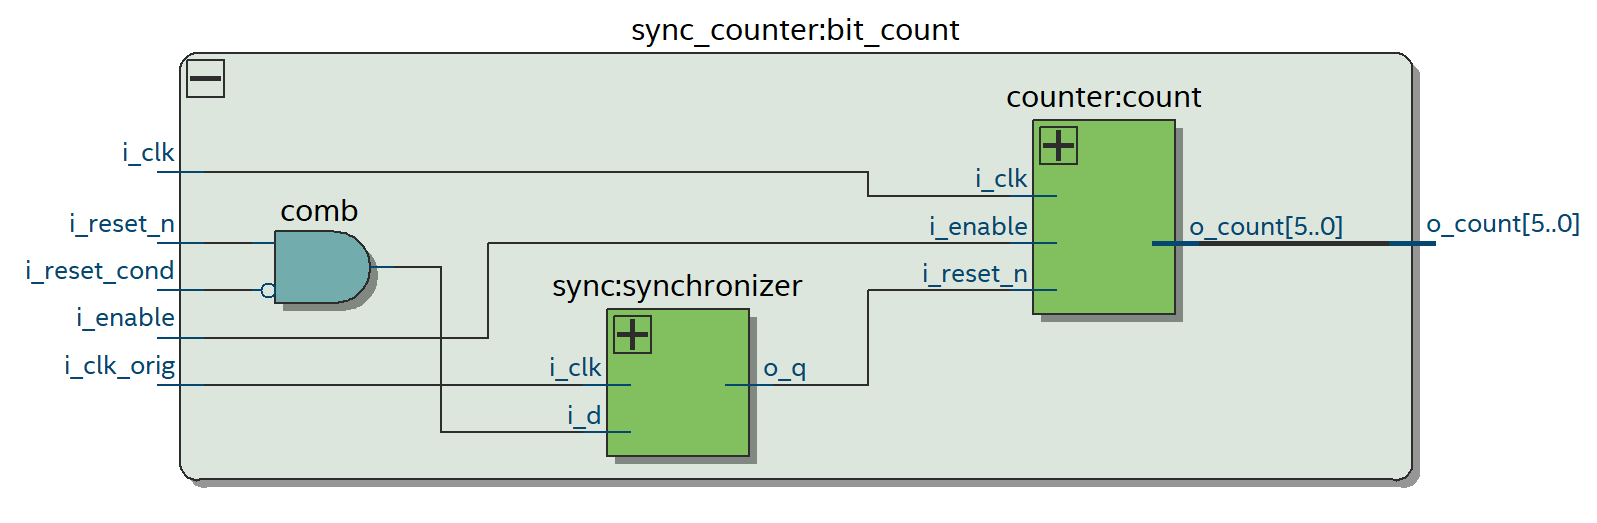
\includegraphics[width=.85\textwidth]{images/block_diagrams/vcr_remote/sync_counter.png}
	\caption{An expanded view of the \code{sync_counter} block \code{bit_count} in \autoref{fig:block_vcr_ir_signal_transcriber_1}.  This module acts like a clock but places a synchronizer between the reset input and the clock reset.  It also adds an extra reset condition \code{i_reset_cond} that is combined with the active low \code{i_reset_n} to also reset the counter when that input is high.}
	\label{fig:block_vcr_sync_counter}
\end{figure}

\begin{figure}[H]
	\centering
	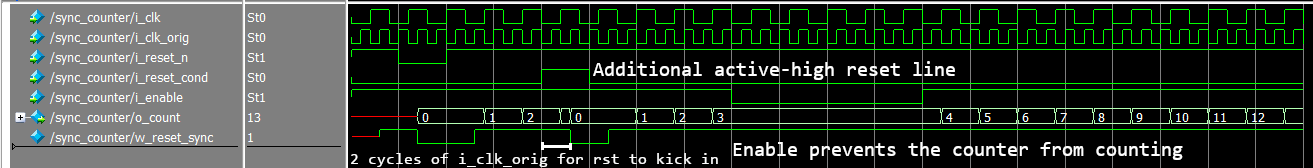
\includegraphics[width=.95\textwidth]{images/sim/vcr_remote/sync_counter.png}
	\caption{Simulation results for the \code{sync_counter} module (see \autoref{lst:sim_vcr_sync_counter} for simulation code).}
\end{figure}

\subsubsection{Counter}

\textbf{Input:} This module reads a clock signal (\code{i_clk}), an enable signal (\code{i_enable}), and an active low reset (\code{i_reset_n}).  
\\ \\
\textbf{Output:} \code{o_count} provides the current value of the counter.
\\ \\
The code for this block is given in \autoref{lst:sv_vcr_counter}.

\begin{figure}[H]
	\centering
	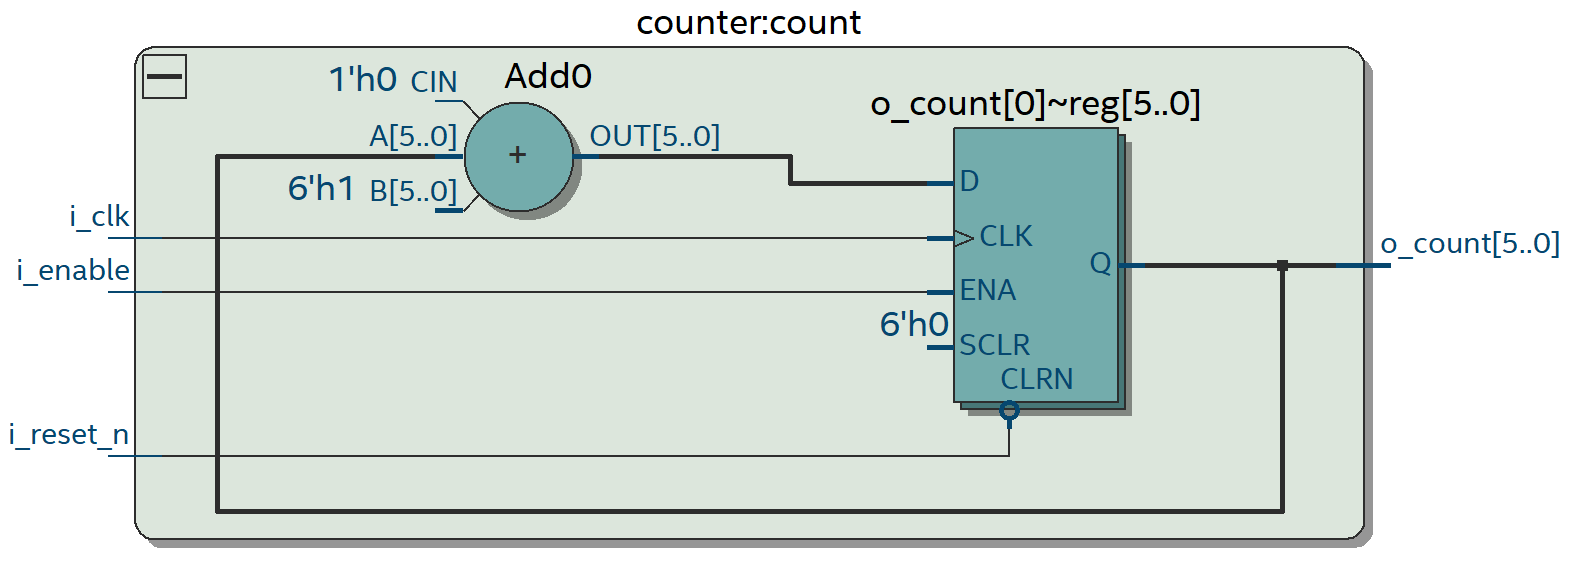
\includegraphics[width=.85\textwidth]{images/block_diagrams/vcr_remote/counter.png}
	\caption{An expanded view of the \code{counter} block \code{count} in \autoref{fig:block_vcr_sync_counter}.  The counter contains D flip-flops with enable and clear inputs that increment the stored value on each rising edge of \code{i_clk}.}
	\label{fig:block_vcr_counter}
\end{figure}

\begin{figure}[H]
	\centering
	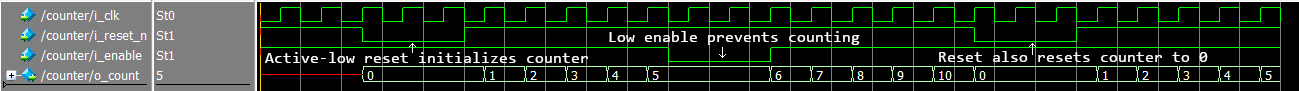
\includegraphics[width=.95\textwidth]{images/sim/vcr_remote/counter.png}
	\caption{Simulation results for the \code{counter} module (see \autoref{lst:sim_vcr_counter} for simulation code).}
\end{figure}

\subsubsection{Synchronizer}

\textbf{Input:} This module reads a clock signal (\code{i_clk}) and a data signal (\code{i_d}).
\\ \\
\textbf{Output:} \code{o_q} provides the synchronized data signal.
\\ \\
The code for this block is given in \autoref{lst:sv_vcr_sync}.

\begin{figure}[H]
	\centering
	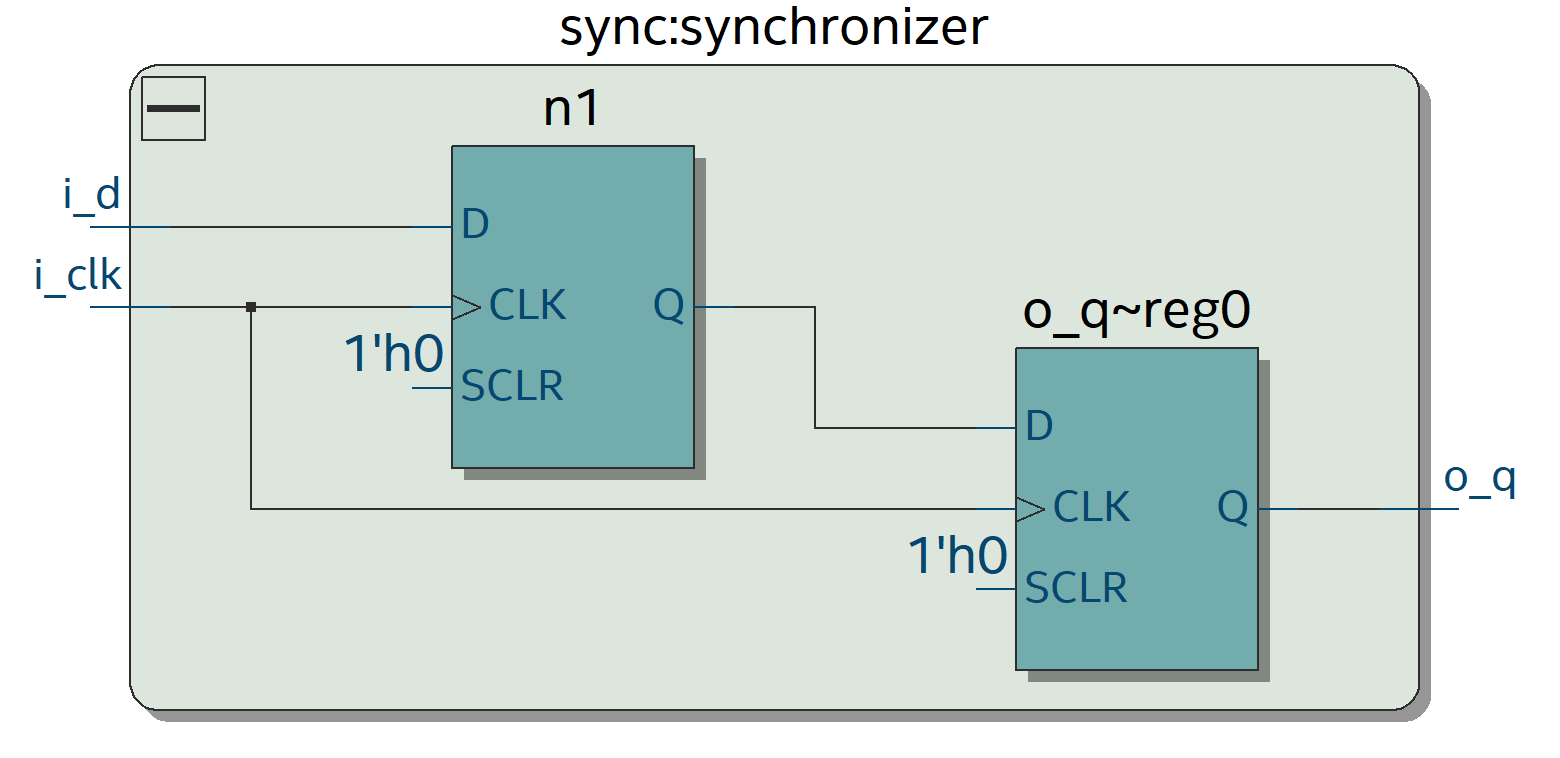
\includegraphics[width=.85\textwidth]{images/block_diagrams/vcr_remote/sync.png}
	\caption{An expanded view of the \code{sync} block \code{synchronizer} in \autoref{fig:block_vcr_sync_counter}.  The synchronizer contains two D flip-flops, forcing the input value \code{i_d} to pass through both (synchronizing with \code{i_clk} in the process) before being output on \code{o_q}.}
	\label{fig:block_vcr_sync}
\end{figure}

\begin{figure}[H]
	\centering
	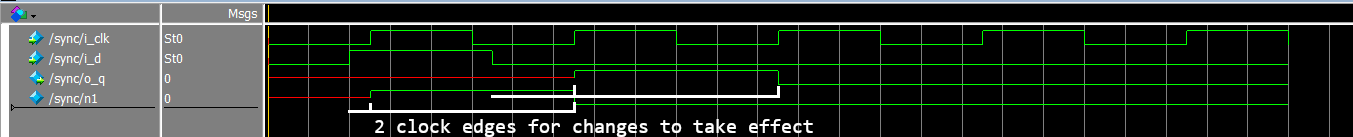
\includegraphics[width=.95\textwidth]{images/sim/vcr_remote/sync.png}
	\caption{Simulation results for the \code{sync} module (see \autoref{lst:sim_vcr_sync} for simulation code).}
\end{figure}

\subsubsection{Shift Register}

\textbf{Input:} This module reads a clock signal (\code{i_clk}), an enable signal (\code{i_enable}), and an active low reset signal (\code{i_reset_n}).  It also has a serial input (\code{i_sin}), a parallel input (\code{i_pin}), and a parallel load signal (\code{i_load}).
\\ \\
\textbf{Output:} \code{o_sout} provides the stored data serially.  \code{o_pout} provides the stored data in a parallel format.
\\ \\
The code for this block is given in \autoref{lst:sv_vcr_shiftreg}.

\begin{figure}[H]
	\centering
	\includegraphics[width=.85\textwidth]{images/block_diagrams/vcr_remote/shiftreg.png}
	\caption{An expanded view of the \code{shiftreg} block \code{bit_store} in \autoref{fig:block_vcr_ir_decoder}.  The shift register uses D flip-flops with enable and clear inputs to store thir value.  If \code{i_load} is low, \code{i_sin} is combined with all of the stored bits without the oldest one and sent to the flip-flops' data inputs.  If \code{i_load} is high, the entirety of \code{i_pin} is sent to those data inputs.}
	\label{fig:block_vcr_shiftreg}
\end{figure}

\begin{figure}[H]
	\centering
	\includegraphics[width=.95\textwidth]{images/sim/vcr_remote/shiftreg.png}
	\caption{Simulation results for the \code{shiftreg} module (see \autoref{lst:sim_vcr_shiftreg} for simulation code).}
\end{figure}

\subsubsection{Checksum Validator}

\textbf{Input:} This module reads a signal (\code{i_data}) for the code to be checked.
\\ \\
\textbf{Output:} \code{o_checksum_valid} indicates whether the code's checksum is valid.
\\ \\
The code for this block is given in \autoref{lst:sv_vcr_checksum_validator}.

\begin{figure}[H]
	\centering
	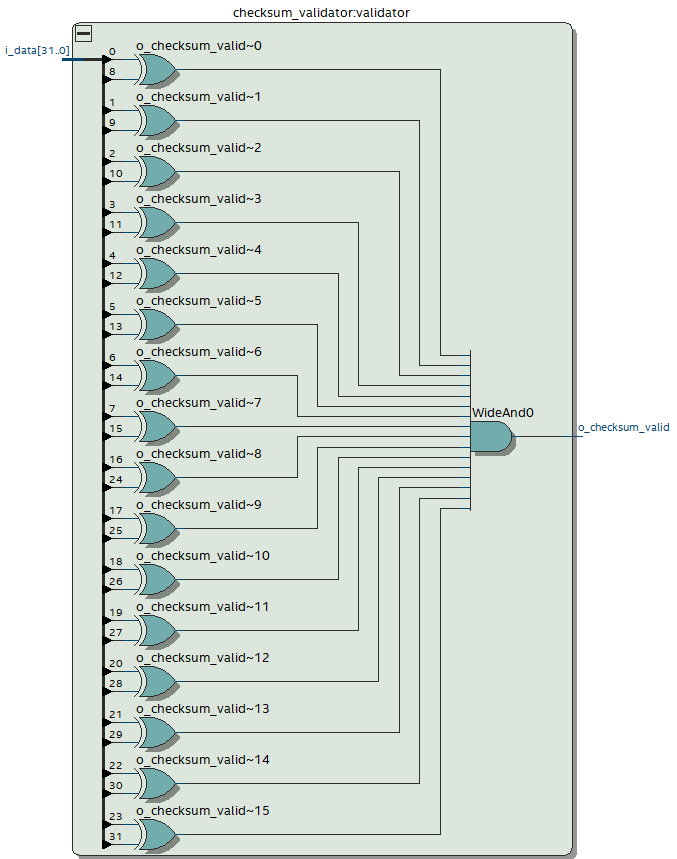
\includegraphics[width=.85\textwidth]{images/block_diagrams/vcr_remote/checksum_validator.png}
	\caption{An expanded view of the \code{checksum_validator} block \code{validator} in \autoref{fig:block_vcr_ir_decoder}.  The validator XORs the first quarter of the code with the second quarter and the third quarter of the code with the fourth.  If the checksum is valid, the result should be a string of all 1s. This is checked by ANDing together the output of all of the XORs.  The result of this (\code{o_checksum_valid}) is 1 if the checksum is valid and 0 if it is invalid.}
	\label{fig:block_vcr_checksum_validator}
\end{figure}

\begin{figure}[H]
	\centering
	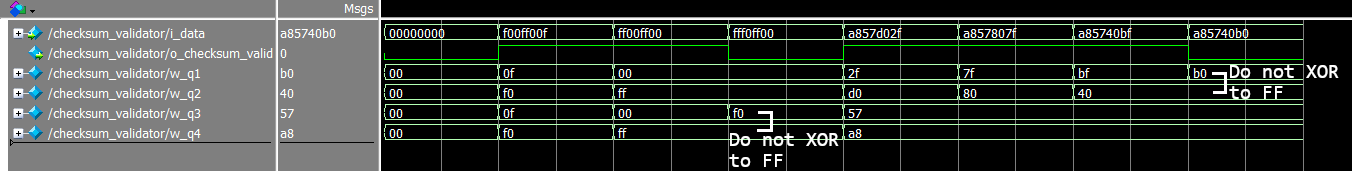
\includegraphics[width=.95\textwidth]{images/sim/vcr_remote/checksum_validator.png}
	\caption{Simulation results for the \code{checksum_validator} module (see \autoref{lst:sim_vcr_checksum_validator} for simulation code).}
\end{figure}

\subsubsection{IR Code Decoder}

\textbf{Input:} This module reads the code to be decoded (\code{i_ir_code}) .
\\ \\
\textbf{Output:} \code{o_decoded} provides the decoded value sent by the remote (a number 0-9).
\\ \\
The code for this block is given in \autoref{lst:sv_vcr_ir_code_decoder}.

\begin{figure}[H]
	\centering
	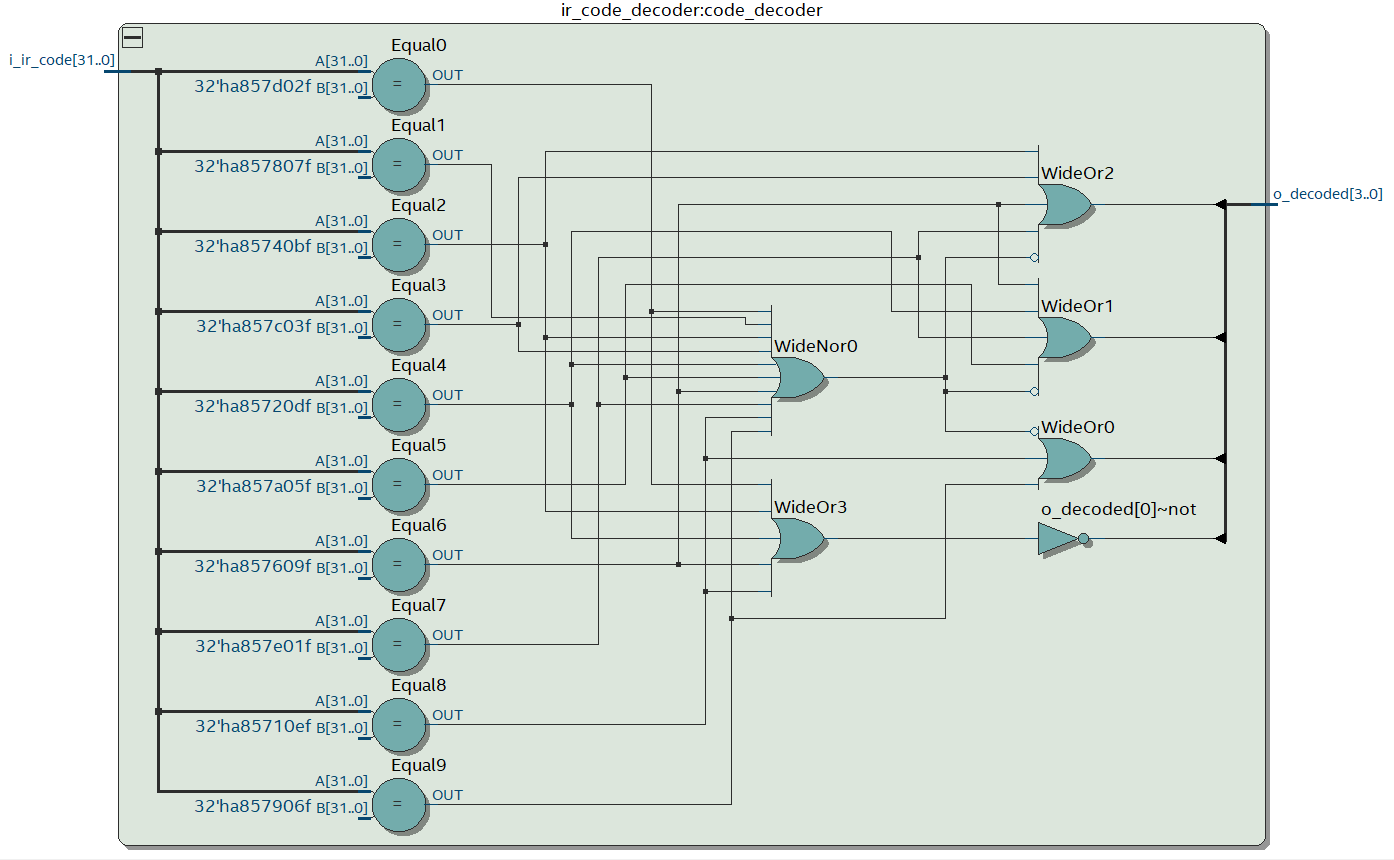
\includegraphics[width=.85\textwidth]{images/block_diagrams/vcr_remote/ir_code_decoder.png}
	\caption{An expanded view of the \code{ir_code_decoder} block \code{code_decoder} in \autoref{fig:block_vcr_ir_decoder}.  On the left, \code{i_ir_code} is checked against each of the possible codes so that the output of the comparators acts as a one-hot encoding of the decoded value.  On the right is the simplified logic which uses these outputs to set the bits of \code{o_decoded} accordingly.}
	\label{fig:block_vcr_ir_code_decoder}
\end{figure}

\begin{figure}[H]
	\centering
	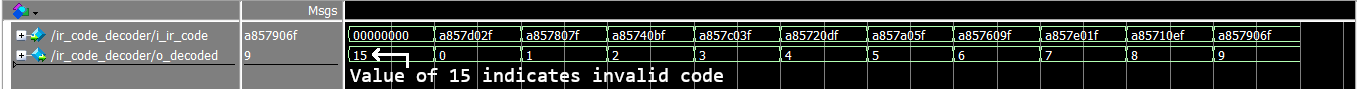
\includegraphics[width=.95\textwidth]{images/sim/vcr_remote/ir_code_decoder.png}
	\caption{Simulation results for the \code{ir_code_decoder} module (see \autoref{lst:sim_vcr_ir_code_decoder} for simulation code).}
\end{figure}


\appendix
\section{SystemVerilog Files}
\filelisting[label=lst:sv_toplevel]{../verilog/final_project.sv}
\filelisting[label=lst:sv_devices_mux]{../verilog/devices_mux.sv}

\subsection{NES Controller Reader}
\filelisting[label=lst:sv_nes_dp_nes]{../verilog/nes/DP_NES.sv}

\subsection{PS2 Keyboard Decoder}
\filelisting[label=lst:sv_ps2_ps_2]{../verilog/ps2/PS_2.v}
\filelisting[label=lst:sv_ps2_data_received]{../verilog/ps2/data_received.v}
\filelisting[label=lst:sv_ps2_sync_ps2]{../verilog/ps2/sync_ps2.sv}
\filelisting[label=lst:sv_ps2_valid]{../verilog/ps2/valid.sv}
\filelisting[label=lst:sv_ps2_compare]{../verilog/ps2/compare.sv}
\filelisting[label=lst:sv_ps2_encounter]{../verilog/ps2/encounter.sv}
\filelisting[label=lst:sv_ps2_sevenseg]{../verilog/ps2/sevenseg.sv}
\filelisting[label=lst:sv_ps2_checker]{../verilog/ps2/checker.v}
\filelisting[label=lst:sv_ps2_message]{../verilog/ps2/message.sv}

\subsection{VCR Remote Decoder}
\filelisting[label=lst:sv_vcr_ir_decoder]{../verilog/vcr_remote/ir_decoder.sv}
\filelisting[label=lst:sv_vcr_ir_signal_transcriber]{../verilog/vcr_remote/ir_signal_transcriber.sv}
\filelisting[label=lst:sv_vcr_sync_counter]{../verilog/vcr_remote/sync_counter.sv}
\filelisting[label=lst:sv_vcr_counter]{../verilog/vcr_remote/counter.sv}
\filelisting[label=lst:sv_vcr_sync]{../verilog/vcr_remote/sync.sv}
\filelisting[label=lst:sv_vcr_shiftreg]{../verilog/vcr_remote/shiftreg.sv}
\filelisting[label=lst:sv_vcr_checksum_validator]{../verilog/vcr_remote/checksum_validator.sv}
\filelisting[label=lst:sv_vcr_ir_code_decoder]{../verilog/vcr_remote/ir_code_decoder.sv}

\section{Simulation Files (Do scripts)}
\filelisting[label=lst:sim_devices_mux]{../do_files/devices_mux.do}

\subsection{NES Controller Reader}

\begin{figure}[H]
  \centering
    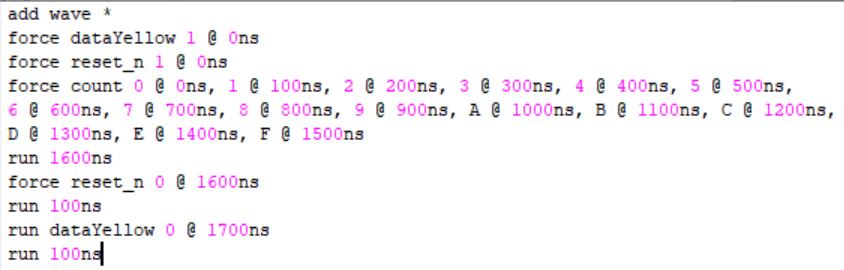
\includegraphics[width=.85\textwidth]{images/ModelSim/nesdo.JPG}
	\caption{NES.do}
    \label{fig:top_level_do}
\end{figure}

\subsection{PS2 Keyboard Decoder}

\subsubsection{\texttt{PS\_2} Module}
\filelisting[label=lst:sim_ps2_ps_2]{../do_files/ps2/PS2.do}

\subsection{VCR Remote Decoder}

\subsubsection{\texttt{ir\_decoder} and \texttt{ir\_signal\_transcriber} Modules}
\filelisting{../do_files/vcr_remote/setup.do}
\filelisting{../do_files/vcr_remote/reset.do}
\filelisting[label=lst:sim_vcr_ir_decoder_0]{../do_files/vcr_remote/0.do}
\filelisting[label=lst:sim_vcr_ir_decoder_1]{../do_files/vcr_remote/1.do}
\filelisting[label=lst:sim_vcr_ir_decoder_2]{../do_files/vcr_remote/2.do}
\filelisting[label=lst:sim_vcr_ir_decoder_3]{../do_files/vcr_remote/3.do}
\filelisting[label=lst:sim_vcr_ir_decoder_4]{../do_files/vcr_remote/4.do}
\filelisting[label=lst:sim_vcr_ir_decoder_5]{../do_files/vcr_remote/5.do}
\filelisting[label=lst:sim_vcr_ir_decoder_6]{../do_files/vcr_remote/6.do}
\filelisting[label=lst:sim_vcr_ir_decoder_7]{../do_files/vcr_remote/7.do}
\filelisting[label=lst:sim_vcr_ir_decoder_8]{../do_files/vcr_remote/8.do}
\filelisting[label=lst:sim_vcr_ir_decoder_9]{../do_files/vcr_remote/9.do}
\filelisting[label=lst:sim_vcr_ir_decoder_sequence]{../do_files/vcr_remote/sequence.do}
\filelisting[label=lst:sim_vcr_ir_decoder_bad_checksum]{../do_files/vcr_remote/bad_checksum.do}

\subsubsection{\texttt{sync\_counter} Module}
\filelisting[label=lst:sim_vcr_sync_counter]{../do_files/vcr_remote/sync_counter.do}

\subsubsection{\texttt{counter} Module}
\filelisting[label=lst:sim_vcr_counter]{../do_files/vcr_remote/counter.do}

\subsubsection{\texttt{sync} Module}
\filelisting[label=lst:sim_vcr_sync]{../do_files/vcr_remote/sync.do}

\subsubsection{\texttt{shiftreg} Module}
\filelisting[label=lst:sim_vcr_shiftreg]{../do_files/vcr_remote/shiftreg.do}

\subsubsection{\texttt{checksum\_validator} Module}
\filelisting[label=lst:sim_vcr_checksum_validator]{../do_files/vcr_remote/checksum_validator.do}

\subsubsection{\texttt{ir\_code\_decoder} Module}
\filelisting[label=lst:sim_vcr_ir_code_decoder]{../do_files/vcr_remote/ir_code_decoder.do}

\section{FPGA Usage Data}

\begin{figure}[ht]
	\centering
	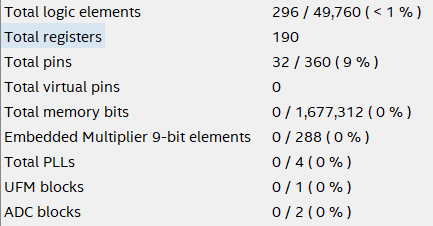
\includegraphics[width=.6\textwidth]{images/fpga_usage.png}
	\caption{FPGA usage data from compilation of project top-level.}
	\label{fig:fpga_usage}
\end{figure}

\printbibliography

\end{document}
